% !TeX spellcheck = en_US
\documentclass[11pt, a4paper]{amsart}

\usepackage[T1]{fontenc}
\usepackage[utf8]{inputenc}
\usepackage{lmodern}
\usepackage{stmaryrd}

% Resume numbering in enumerate
% https://tex.stackexchange.com/questions/1669/resuming-a-list
\usepackage{enumitem}


% % % % % % % % % % % % %
% Loading 'commands' file
% Master commands file
% Dependencies: none

% Text
\newcommand{\OneHalf}{{\textstyle\frac{1}{2}}}
\newcommand{\OneQuart}{{\textstyle\frac{1}{4}}}

% Hyphenation.
\hyphenation{Thurs-ton}
\hyphenation{mo-no-poles}
\hyphenation{sur-ger-y}

%-------------------------------------------------------------------------------

% Pairs of openings and closures
\newcommand{\set}[1]{\mathchoice%
  {\left\lbrace #1 \right\rbrace}%
  {\lbrace #1 \rbrace}%
  {\lbrace #1 \rbrace}%
  {\lbrace #1 \rbrace}%
}
\newcommand{\setc}[2]{\mathchoice%
  {\left\lbrace #1 \, \middle\vert \, #2 \right\rbrace}%
  {\lbrace #1 \, \vert \, #2 \rbrace}%
  {\lbrace #1 \, \vert \, #2 \rbrace}%
  {\lbrace #1 \, \vert \, #2 \rbrace}%
%  {\left\lbrace #1 \, \colon \, #2 \right\rbrace}%
%  {\lbrace #1 \, \colon \, #2 \rbrace}%
%  {\lbrace #1 \, \colon \, #2 \rbrace}%
%  {\lbrace #1 \, \colon \, #2 \rbrace}%
}
\newcommand{\paren}[1]{\mathchoice%
  {\left( #1 \right)}%
  {( #1 )}%
  {( #1 )}%
  {( #1 )}%
}
\newcommand{\brac}[1]{\mathchoice%
  {\left[ #1 \right]}%
  {[ #1 ]}%
  {[ #1 ]}%
  {[ #1 ]}%
}
\newcommand{\abs}[1]{\mathchoice%
  {\left\lvert #1 \right\rvert}%
  {\lvert #1 \rvert}%
  {\lvert #1 \rvert}%
  {\lvert #1 \rvert}%
}
\newcommand{\norm}[1]{\mathchoice%
  {\left\lVert #1 \right\rVert}%
  {\lVert #1 \rVert}%
  {\lVert #1 \rVert}%
  {\lVert #1 \rVert}%
}

% Synonyms for symbols
\newcommand{\eps}{\epsilon}                  % mathord
\newcommand{\veps}{\varepsilon}              % mathord
%\renewcommand{\phi}{\varphi}                 % mathord
\newcommand{\vphi}{\varphi}                  % mathord
\newcommand{\eset}{\varnothing}             % mathord
%\newcommand{\eset}{\emptyset}                % mathord

\newcommand{\dirsum}{\oplus}                 % mathbin
\newcommand{\bigdirsum}{\bigoplus}           % mathop
\newcommand{\tensor}{\otimes}                % mathbin
\newcommand{\bigtensor}{\bigotimes}          % mathop
\newcommand{\union}{\cup}                    % mathbin
\newcommand{\bigunion}{\bigcup}              % mathop
\newcommand{\intersect}{\cap}                % mathbin
\newcommand{\bigintersect}{\bigcap}          % mathop

\newcommand{\comp}{\circ}                    % mathbin
\newcommand{\cross}{\times}                  % mathbin

\newcommand{\isom}{\cong}                    % mathrel
\newcommand{\qisom}{\simeq}                  % mathrel
\newcommand{\nisom}{\ncong}                  % mathrel
\newcommand{\nqisom}{\not\simeq}             % mathrel
\newcommand{\superset}{\supset}              % mathrel
\newcommand{\contains}{\ni}                  % mathrel

% Special sets
\newcommand{\numset}[1]{\mathbb{#1}}
\newcommand{\N}{\numset{N}}
\newcommand{\Z}{\numset{Z}}
\newcommand{\Zpos}{\Z_{\geq 0}}
\newcommand{\Q}{\numset{Q}}
\newcommand{\R}{\numset{R}}
\newcommand{\C}{\numset{C}}
\newcommand{\F}[1]{\numset{F}_{#1}}
\newcommand{\cycgrp}[1]{\Z / #1 \Z}
\newcommand{\field}[1]{\mathbf{#1}}
\renewcommand{\j}{\field{j}}
\renewcommand{\k}{\field{k}}

% Punctuation
%\newcommand{\co}{\colon}
%\newcommand{\semico}{;\penalty 300}
\newcommand{\scolon}{; \penalty 300}

% Common operators
\DeclareMathOperator{\id}{id}
\DeclareMathOperator{\Id}{Id}
\DeclareMathOperator{\sgn}{sgn}
\DeclareMathOperator{\Ker}{Ker}
\DeclareMathOperator{\Coker}{Coker}
\DeclareMathOperator{\im}{Im} % Image
\renewcommand{\Im}{\im}
\DeclareMathOperator{\homgy}{H} % Homology
\DeclareMathOperator{\Hom}{Hom} % Homomorphism
\DeclareMathOperator{\Cone}{Cone}
\DeclareMathOperator{\rk}{rk} % Rank
\DeclareMathOperator{\Hochsch}{HH} % Hochschild homology
\newcommand{\MCG}{\mathit{MCG}} % Mapping class group
\DeclareMathOperator{\Neg}{neg}


% Dodecahedral group
\newcommand{\Dod}{\mathrm{Dod}}

% Matrix groups
\newcommand{\matrixgrp}[1]{\mathrm{#1}}
\newcommand{\GL}{\matrixgrp{GL}}
\newcommand{\SL}{\matrixgrp{SL}}
\newcommand{\SO}{\matrixgrp{SO}}
\newcommand{\SU}{\matrixgrp{SU}}
\newcommand{\Sp}{\matrixgrp{Sp}}
\newcommand{\ISO}{\matrixgrp{ISO}}


% Lie algebras
\newcommand{\fsl}{\mathfrak{sl}}
\newcommand{\sltwo}{\fsl_2}
\newcommand{\fg}{\mathfrak g}
\newcommand{\fgl}{\mathfrak{gl}}
\newcommand{\gloneone}{\fgl_{1|1}}

% Basic topology
\newcommand{\torus}{\mathbb{T}}
\newcommand{\bdy}{\partial} % mathord
\newcommand{\connsum}{\mathbin{\#}} % Originally mathord
\newcommand{\bigconnsum}{\mathop{\mathchoice%
    {\vcenter{\hbox{\LARGE $\#$}}}
    {\vcenter{\hbox{\large $\#$}}}
    {\vcenter{\hbox{\footnotesize $\#$}}}
    {\vcenter{\hbox{\scriptsize $\#$}}}
  }}
\newcommand{\bdysum}{\mathbin{\natural}} % Originally mathord
\newcommand{\bigbdysum}{\mathop{\mathchoice%
    {\vcenter{\hbox{\LARGE $\natural$}}}
    {\vcenter{\hbox{\large $\natural$}}}
    {\vcenter{\hbox{\footnotesize $\natural$}}}
    {\vcenter{\hbox{\scriptsize $\natural$}}}
  }}
\DeclareMathOperator{\Sym}{Sym}
\newcommand{\unknot}{\mathord{\bigcirc}} % Originally mathbin
\newcommand{\quasialt}{\mathcal{Q}} % Quasi-alternating links
\newcommand{\QHS}{{\Q}\mathit{HS}^3}
\newcommand{\ZHS}{{\Z}\mathit{HS}^3}
\newcommand{\nbhd}[1]{\nu (#1)}

% interior of a subspace
\DeclareMathOperator{\interior}{int}


% Spheres, disks, ...
\newcommand{\sphere}[1]{{S}^{#1}}
\newcommand{\disk}[1]{{D}^{#1}}
\newcommand{\ball}[1]{{B}^{#1}}
\newcommand{\interval}{{I}}
\newcommand{\RP}[1]{\mathbb{RP}^{#1}}
\newcommand{\CP}[1]{\mathbb{CP}^{#1}}

% Point
\newcommand{\point}{\textup{pt}}

\newcommand{\laurent}{\ZZ[t, t^{-1}]}
% Blanchfield
\newcommand{\Bl}{\operatorname{Bl}}

% Shortcuts for blackboard letters
\newcommand{\ZZ}{\mathbb{Z}}
\newcommand{\QQ}{\mathbb{Q}}
\newcommand{\RR}{\mathbb{R}}
\newcommand{\CC}{\mathbb{C}}
\newcommand{\HH}{\mathbb{H}}

% Free groups
\DeclareMathOperator{\Fr}{Fr}

% (Twist) spinning knots
\newcommand{\Spin}{\tau}


% % % % % % % % % % % %
% Loading TeX packages

\usepackage[american]{babel}
\usepackage[babel, final]{microtype}
\usepackage{amssymb}
\usepackage[all]{xy}

\usepackage{mathtools}

\usepackage{ifpdf}
\usepackage{comment}
\usepackage{multirow}

\usepackage[pdftex, dvipsnames]{xcolor}
\usepackage[pdftex, final]{graphicx}
\usepackage{caption}
\usepackage{pinlabel}
\usepackage[pdftex,%
    a4paper,%
    includehead,%
    includefoot,%
    nomarginpar,%
    lmargin=1.9cm,%
    rmargin=1.9cm,%
    tmargin=1in,%
    bmargin=1in,%
]{geometry}
\usepackage[pdftex,%
    final,%
    colorlinks=true,%
    linkcolor={red!45!black},%
    citecolor=NavyBlue,%
    filecolor=NavyBlue,%
    menucolor=NavyBlue,%
    urlcolor={blue!45!black},%
    bookmarks=true,%
    bookmarksdepth=3,%
    bookmarksnumbered=true,%
    bookmarksopen=true,%
    bookmarksopenlevel=2,%
]{hyperref}
\hypersetup{
    pdftitle={Word Embeddings Seminar Program},
    pdfauthor={Ruppik},
    pdfsubject={Word embedding},
    pdfkeywords={Word embeddings, Natural Language Processing}
}

\usepackage{cleveref}

\usepackage{float}

% Indentation of footnotes
\usepackage[hang,flushmargin]{footmisc}




%~~~~~~~~~~~~~~~~~~ table of contents (toc)

% Using this ad-hoc solution from
% https://tex.stackexchange.com/questions/51760/table-of-contents-with-indents-and-dots
% because most toc packages are not compatible
% with amsart

\makeatletter
\def\@tocline#1#2#3#4#5#6#7{\relax
  \ifnum #1>\c@tocdepth % then omit
  \else
    \par \addpenalty\@secpenalty\addvspace{#2}%
    \begingroup \hyphenpenalty\@M
    \@ifempty{#4}{%
      \@tempdima\csname r@tocindent\number#1\endcsname\relax
    }{%
      \@tempdima#4\relax
    }%
    \parindent\z@ \leftskip#3\relax \advance\leftskip\@tempdima\relax
    \rightskip\@pnumwidth plus4em \parfillskip-\@pnumwidth
    #5\leavevmode\hskip-\@tempdima
      \ifcase #1
       \or\or \hskip 1em \or \hskip 2em \else \hskip 3em \fi%
      #6\nobreak\relax
    \dotfill\hbox to\@pnumwidth{\@tocpagenum{#7}}\par
    \nobreak
    \endgroup
  \fi}
\makeatother

%~~~~~~~~~~~~~~~~~~





%~~~~~~~~~~~~~~~~~~ bibliography
\usepackage{csquotes}
\usepackage[
	backend=biber,
	style=alphabetic,
	sorting=nyt,
	giveninits=true,
	maxnames=10,
	%articlein=false,
	url=false,
	backref=true
]{biblatex}
\DefineBibliographyStrings{english}{
  backrefpage={$\uparrow$},
  backrefpages={$\uparrow$}
}

\addbibresource{references.bib}

\renewcommand*{\bibfont}{\small}
%\renewbibmacro{in:}{%
%	\ifentrytype{article}{}{\printtext{\bibstring{in}\intitlepunct}}}

\renewcommand{\mkbibnamegiven}[1]{\textsc{#1}}
\renewcommand{\mkbibnamefamily}[1]{\textsc{#1}}
\renewcommand{\mkbibnameprefix}[1]{\textsc{#1}}
\renewcommand{\mkbibnamesuffix}[1]{\textsc{#1}}

\DeclareFieldFormat[article,incollection,inproceedings]{title}{#1}
\DeclareFieldFormat[unpublished]{title}{\textit{#1}}



%~~~~~~~~~~~~~~~~~~


\usepackage{tikz}
\usetikzlibrary{tikzmark}
\usepackage{tikz-cd}

\makeatletter
\g@addto@macro\@floatboxreset\centering
\makeatother

\def\mathcenter#1{%
  \vcenter{\hbox{$#1$}}%
}

\allowdisplaybreaks[4]

\addto\extrasamerican{%
  \def\sectionautorefname{Section}%
  \def\subsectionautorefname{Section}%
  \def\subsubsectionautorefname{Section}%
}

\let\fullref\autoref

\newtheorem{theorem}{Theorem}[section]
\newtheorem{conjecture}{Conjecture}[section]
\newtheorem{corollary}{Corollary}[section]
\newtheorem{proposition}{Proposition}[section]
\newtheorem{lemma}{Lemma}[section]
\newtheorem*{geometric-theorem}{Geometric Input Theorem}

\theoremstyle{definition}
\newtheorem*{convention}{Conventions}
\newtheorem{definition}{Definition}[section]
\newtheorem{example}{Example}[section]
\newtheorem{remark}{Remark}[section]
\newtheorem{question}{Question}[section]
\newtheorem*{claim}{Claim}

\makeatletter
\let\c@conjecture=\c@theorem
\let\c@corollary=\c@theorem
\let\c@proposition=\c@theorem
\let\c@lemma=\c@theorem
\let\c@definition=\c@theorem
\let\c@example=\c@theorem
\let\c@remark=\c@theorem
\let\c@equation\c@theorem
\makeatother

\def\makeautorefname#1#2{\expandafter\def\csname#1autorefname\endcsname{#2}}
\makeautorefname{theorem}{Theorem}%
\makeautorefname{conjecture}{Conjecture}%
\makeautorefname{corollary}{Corollary}%
\makeautorefname{proposition}{Proposition}%
\makeautorefname{lemma}{Lemma}%
\makeautorefname{definition}{Definition}%
\makeautorefname{example}{Example}%
\makeautorefname{remark}{Remark}%
\makeautorefname{question}{Question}%
\makeautorefname{claim}{Claim}

\numberwithin{equation}{section}

\newcommand*{\Alphabet}{ABCDEFGHIJKLMNOPQRSTUVWXYZ1234567890}
\newcommand*{\alphabet}{abcdefghijklmnopqrstuvwxyz1234567890}
\newlength\fcaph
\newlength\fdesc
\newlength\factualfontsize
\settoheight{\fcaph}{\footnotesize \Alphabet}
\settodepth{\fdesc}{\footnotesize \Alphabet \alphabet}
\setlength{\factualfontsize}{\dimexpr\fcaph+\fdesc\relax}

% Comments
\numberwithin{equation}{section}
\newcounter{commentcounter}
\newcommand{\commentb}[1]{\stepcounter{commentcounter}
	\textbf{Comment \arabic{commentcounter} (by B.)}:
	{\textcolor{blue}{#1}} }
\newcommand{\commentm}[1]{\stepcounter{commentcounter}
	\textbf{Comment \arabic{commentcounter} (by M.)}:
	{\textcolor{ForestGreen}{#1}} }
\newcommand{\commentr}[1]{\stepcounter{commentcounter}
	\textbf{Comment \arabic{commentcounter} (by R.)}:
	{\textcolor{orange}{#1}} }
\newcommand{\comments}[1]{\stepcounter{commentcounter}
	\textbf{Comment \arabic{commentcounter} (by S.)}:
	{\textcolor{BlueGreen}{#1}} }
\newcommand{\commentv}[1]{\stepcounter{commentcounter}
	\textbf{Comment \arabic{commentcounter} (by V.)}:
	{\textcolor{purple}{#1}} }
	

\newcommand{\missingref}{\textcolor{orange}{[Ref]}}

% Large / for quotients
\newcommand{\bigslant}[2]{{\raisebox{.2em}{$#1$}\left/\raisebox{-.2em}{$#2$}\right.}}


\newcommand{\TODO}{\textcolor{magenta}{TODO }}


% Definitions of the algebraic
% and geometric sets for the 
% last part of the paper
\newcommand{\Alg}{\texttt{\textup{Alg}}}
\newcommand{\Man}{\texttt{\textup{Man}}}
\newcommand{\Diag}{\texttt{\textup{Diag}}}


% booktabs package for the \toprule, \midrule, \bottomrule commands in tables
\usepackage{booktabs}

\usepackage[htt]{hyphenat}

\usepackage{tabularx}
\usepackage{listings}

% Text formatted as language model generation
% https://tex.stackexchange.com/questions/36030/how-to-make-a-single-word-look-as-some-code
% \usepackage{xcolor} % xcolor package is already imported in the commands.tex file
\definecolor{light-gray}{gray}{0.95}
\newcommand{\generatedtext}[1]{\colorbox{light-gray}{{#1}}} % Text formatted as code


\title{Word Embedding Spaces}

% % % % % % % % % % % % %
% Contact information
% % % % % % % % % % % % %

\author{Benjamin Matthias Ruppik}
\address{Dialog Systems and Machine Learning Group, Heinrich-Heine-University D{\"u}sseldorf, Germany}
\email{\href{mailto:benjamin.ruppik@hhu.de}{benjamin.ruppik@hhu.de}}
\urladdr{\url{http://bruppik.de}}

\keywords{
    Natural Language Processing, Word embeddings, Dialog Systems, Topological Data Analysis.
    \hfill
    Date: \today
}


%%%%%%%%%%%%%%%%%%%%%%%%%%%%%%%%%%
% WATERMARK
%%%%%%%%%%%%%%%%%%%%%%%%%%%%%%%%%%
\usepackage{draftwatermark}

\usepackage[yyyymmdd,hhmmss]{datetime}
\usepackage[style=iso]{datetime2}

\SetWatermarkText{Compiled on \today\ at \currenttime}
\SetWatermarkColor[gray]{0.9}
\SetWatermarkFontSize{1cm}
\SetWatermarkAngle{90}
\SetWatermarkHorCenter{20cm}
%%%%%%%%%%%%%%%%%%%%%%%%%%%%%%%%%%

\usepackage{pdfpages}

% % % % % % % % % % % % % % % %
% Conventions:
%
% - Use American spelling, in particular:
% stabilization, realization, canceled, canceling, 
% labeled, labeling
%
% - For inverses of group elements, write it out as
% ^{-1} instead of using overlines
%

% LaTeX conventions:
%
% - Each sentence should start a new line
% (this makes comparing different versions easier)
%
% - Use \ldots instead of ...
%
% - Insert figures directly underneath paragraph in which 
% main reference is located
% 


%%%%%%%%%%%%%%%%%%%%%%%%%%%%%%%%
%%%%%%%%%%%%%%%%%%%%%%%%%%%%%%%%
\begin{document}

\begin{abstract}
	Word embedding spaces are a powerful tool for natural language processing (NLP), as they allow us to represent words as real-valued vectors that capture their semantic and syntactic properties.
	These ideas fit into the more general framework of \emph{Representation Learning}, a way to automatically learn features from data.
	In this seminar, we will explore different methods for creating and using word embedding spaces, from static models like word2vec and fastText, to contextual models like ELMo, BERT, RoBERTa, and GPT.
	We will also analyse the geometry and topology of word embedding spaces, and how they relate to linguistic phenomena such as analogy, similarity and compositionality.
	Finally, we will discuss some applications of word embeddings in task-oriented dialogue systems, such as intent detection, slot filling and response generation.
	We will also introduce some current aligned language models such as InstructGPT and ChatGPT that leverage word embeddings for generating natural and engaging conversations.
\end{abstract}

\maketitle

This document contains extended notes for the Seminar ``Word Embedding Spaces'', Heinrich-Heine-University D{\"u}sseldorf, Summer Term 2023.

% --------------------------------- %
\section*{Organization}
% --------------------------------- %

\begin{itemize}
    \item \textbf{Summer Term 2023 at HHU:} 
     ``Master's Seminar on Word Embedding Spaces''
    \item Wednesday; 12:30 -- 14:00; from 05.04.2023 to 12.07.2023; Location: Gebäude 25.22 - 2522.U1.72
    \item \href{https://docs.google.com/spreadsheets/d/1V-d-QuJIUniPq9q-Xviu_TdLZHlW_xzBTqhDX_lIG9w/edit?usp=sharing}{Schedule on Google Sheets}
    \item Lecture course repository: \url{https://github.com/ben300694/word-embeddings}
    \item Live stream on WebEx will probably be available for registered participants.
    \item \textbf{Requirements for receiving credit points:}
    \begin{itemize}
        \item Active participation in the seminar sessions. 
        \begin{itemize}
        	\item Active participation in the seminar sessions means that students are expected to attend all the sessions, read the assigned materials in advance, and engage in constructive discussions with their peers and the instructor.
        	\item Active participation also means that students should ask relevant questions, share their opinions and insights, and provide constructive feedback to their classmates’ presentations.
        \end{itemize}
        \item Delivery of one scientific presentation.
        \begin{itemize}
        	\item The topics will be assigned by me at the beginning of the semester.
        	Students should contact me as soon as possible to choose their preferred topic from the available list.
        	\item Before giving their presentation in class, students must schedule a meeting with me to show a draft of their slides and receive feedback and suggestions for improvement.
        	\item The presentations should be clear, concise and well-structured.
        	They should include an introduction, a literature review, a main argument, and a conclusion.
        	They should also cite relevant sources and use appropriate visual aids.
        \end{itemize}
        \item Submission of a  \LaTeX-file and compiled PDF of an extended abstract:
        \begin{itemize}
        	\item No more than 2 pages.
        	\item Using the \href{https://www.overleaf.com/latex/templates/acl-2020-proceedings-template/zsrkcwjptpcd}{ACL Overleaf template}.
        	\item Including relevant references to scientific literature.
        \end{itemize}
    \end{itemize}
    \item \textbf{Formal Prerequisites:} None
    \item \textbf{Recommended Prerequisites:}
    Background in deep learning,
    linear algebra.
\end{itemize}

% % % % % % % % % % % % % % % % % % %
\subsection*{Policy on AI writing assistants}

AI writing assistants, such as chatbots or language models like ChatGPT \cite{ChatGPT} and GitHub Copilot, may be used as a tool to enhance writing skills and productivity.
However, it is important to note that the final product submitted must be original work and properly cited if using any direct quotes or paraphrased material.
Plagiarism, including use of AI writing assistance without proper citation, will not be tolerated and is a violation of academic honesty.

Please have a look thoughts collected on the website \href{https://platform.openai.com/docs/chatgpt-education}{Educator considerations for ChatGPT}.

\clearpage
% --------------------------------- %
\section{Introduction}
\label{sec:intro}
% --------------------------------- %

In a \emph{word embedding} we encode language by associating to a word $w$ a point or vector $v_{w} \in \RR^{n}$ in some ambient space, such that words which have similar meaning are close together in the space.
When words are modelled as vectors or points in an ambient high-dimensional space, this is called an \emph{embedding}.

% Forcing figure placement here by \usepackage{float} and [H] option
% https://tex.stackexchange.com/questions/8625/force-figure-placement-in-text
\begin{figure}[H]
    \centering
    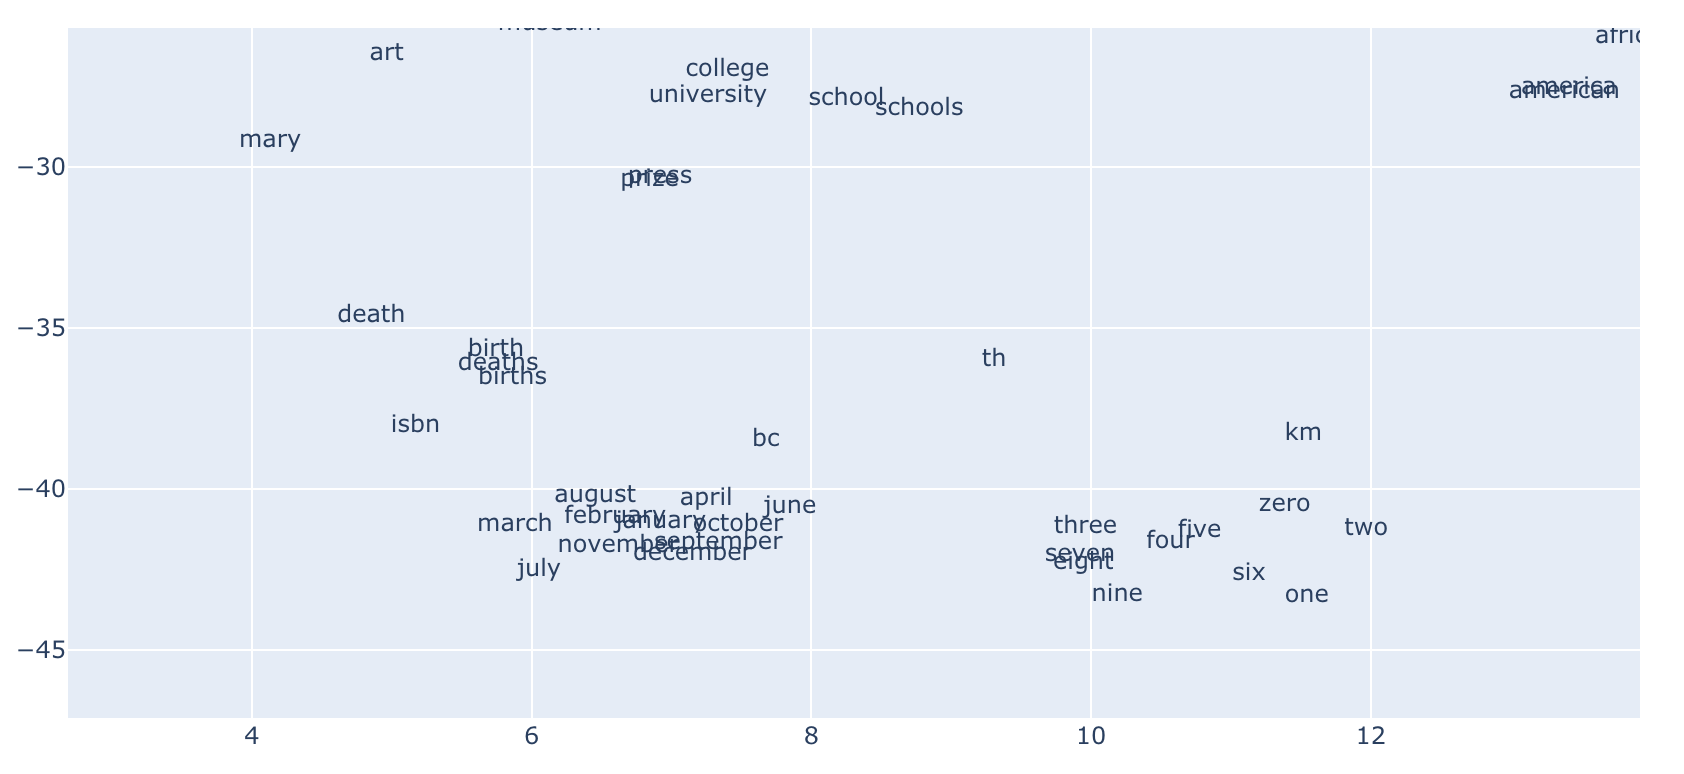
\includegraphics[width=\linewidth]{figures/fastText_tSNE_screenshot.png}
    \caption{
    	Some of the word vectors in a 100 dimensional fastText embedding trained on a Wikipedia corpus; projected to 2 dimensions using $t$-SNE.
    }
    \label{fig:fastText_tSNE}
\end{figure}

Words which are used in similar contexts usually have similar meanings.\footnote{This is not always true, as the words `good' and `bad' demonstrate, more on this below.}
The \emph{distributional hypothesis} states that words which frequently appear in similar contexts have similar meanings.
There is \emph{first-order co-occurence}, also called \emph{syntagmatic association}, if the words are typically nearby each other; for example: `wrote' and `book', `wrote' and `poem'.
We also observe \emph{second order co-occurence}, called \emph{paradigmatic association}, if the words have similar neighbors; for example: `wrote' and `said', `wrote' and `remarked'.

This makes it possible to acquire meaningful representations from unlabeled data -- and there is lots of unlabeled data, e.g., in the form of text from Wikipedia, books, or news headlines.
Thus, we can make both \emph{distributed} and \emph{distributional representations}:
Distributional means that it is based on counts of words in context;
distributed means that the representation is vector based.

The task of finding good word embeddings becomes hard because there are many subtleties in the usage of words in natural language.
Words (or \emph{lemmas}) like `mole' can have multiple meanings, which are its \emph{word senses}; a word which has multiple meanings is \emph{polysemous}.
The embedding should also be able to capture concepts such as \emph{synonyms} (words have the same meaning in many or all contexts) and \emph{antonyms} (the word senses are opposites with respect to one feature of the meaning), \emph{similarity}, \emph{relatedness}, \emph{connotation} or \emph{sentiment}.
There is usually a \emph{super-subordinate} relation (also called \emph{hyperonymy}, \emph{hyponymy} or ``is-a'' relation).
On the other hand, \emph{stop words} like `a', `the', `is', `are', `and' are so commonly used that they carry very little useful information.

There is a big difference between \emph{static} and \emph{contextualized} embeddings:
In a \emph{static embedding} (\Cref{sec:static_word_embeddings}) there is one fixed embedding for each word in the vocabulary.
In a \emph{contextual embedding} (\Cref{sec:contextual_word_embeddings}) the vector we associate to a word is different if it is used in a different context.

We will also talk about how one can systematically evaluate the quality of a word embedding.
In \emph{extrinsic evaluation}, we use a word embedding for a specific downstream task and measure whether it increases performance.
\emph{Intrinsic evaluation} is a harder challenge.

% % % % % % % % % % % % % % % % % % %
\subsection{General References and Links}
\label{sec:general_references}

\begin{itemize}
    \item For a general introduction to NLP see the book \cite{jurafsky2009speech}.
    A \href{https://web.stanford.edu/~jurafsky/slp3/}{draft of the 3rd edition} is available on the authors' website.
    For the topic of word embeddings, Chapter 6 on ``Vector Semantics and Embeddings'' is particularly relevant.
    There are corresponding \href{https://web.stanford.edu/~jurafsky/slp3/slides/6_Vector_Apr18_2021.pdf}{slides} as well.

    \item \cite[Chp.~14]{eisenstein2019introduction} on ``Distributional and Distributed Semantics'';
    draft available \href{https://github.com/jacobeisenstein/gt-nlp-class/blob/master/notes/eisenstein-nlp-notes.pdf}{here}.

    \item \href{https://www.cs.hhu.de/fileadmin/redaktion/Fakultaeten/Mathematisch-Naturwissenschaftliche_Fakultaet/Informatik/Dialog_Systems_and_Machine_Learning/20190705_word_embeddings.pdf}{Michael Heck's slides (2019)} on the Space of Word Embeddings.
    
    \item \href{https://lena-voita.github.io/nlp_course}{Lena Voita's NLP Course For You}, in particular the lesson on \href{https://lena-voita.github.io/nlp_course/word_embeddings}{Word Embeddings} and the lesson on \href{https://lena-voita.github.io/nlp_course/seq2seq_and_attention.html}{Sequence to Sequence (seq2seq) and Attention}.
    
    \item \href{https://youtube.com/playlist?list=PL75e0qA87dlG-za8eLI6t0_Pbxafk-cxb}{Rasa Algorithm Whiteboard} YouTube playlist.
    
    \item \href{https://www.youtube.com/c/aicoffeebreak}{AI Coffee Break with Letitia} YouTube channel.
\end{itemize}

% % % % % % % % % % % % % % % %
\subsubsection{Acknowledgments}

The content of this document is based on the seminar ``Word Embedding Spaces'' run at Heinrich-Heine-University Düsseldorf in the Summer Term 2022 and 2023.
I am grateful for the suggestions and feedback collected during the sessions. Thank you to Milica Gašić, Chris Geishauser, Michael Heck for very helpful additional input. \\
Parts of the current notes are based on the final reports written by the following students:
\begin{itemize}
	\item Nick Rucks: fastText and GloVe
	\item Lukas Rücker: Sequence to Sequence and Recurrent Methods
	\item Benedikt Prusas, Benedikt Jung: Transformers
	\item Thanh Nam Le, Michail Angelos Severino Theoktistou: Masked Language Models and BERT
\end{itemize}

A small portion of these learning materials was drafted with the help of AI writing assistants such as ChatGPT, GitHub Copilot and Microsoft Bing Search Chat Mode.
The majority of the content was written by human experts and all content has been manually edited and fact checked for accuracy.
Please see \Cref{appendix:prompts} for further details on how generative AI was used in our writing and editing process. \\

%~~~~~~~~~~~~~~~~~~~~~~~~~~~~~~~~~~~~~~~~~~%
\section{Background and Static Word Embeddings}
\label{sec:static_word_embeddings}
%~~~~~~~~~~~~~~~~~~~~~~~~~~~~~~~~~~~~~~~~~~%


% % % % % % % % % % % % % % % % % % %
\subsection{Frequency based methods}

Frequency based word embedding methods are one of the simplest and oldest approaches to word embedding.
They are based on determining the frequencies of words in documents or sentences, and using them to create vector representations for words.
Frequency based methods can be divided into three main types: count vectors, TF-IDF, and co-occurrence matrices.
These methods have some advantages, such as being easy to understand and implement, but also some disadvantages, such as being sparse, high-dimensional, and ignoring the semantic context of words.

Here are a few key-words and terminology that you should know about:
\begin{itemize}
	\item Co-occurence counts;
	\item Term-document matrix: each document is represented by a vector of word counts;
	\item \textbf{T}erm \textbf{F}requency -- \textbf{I}nverse \textbf{D}ocument \textbf{F}requency (TF-IDF):
	sparse vectors, words are represented as a simple function of the counts of neighbors;
	\item \textbf{P}ointwise \textbf{P}ositive \textbf{M}utual \textbf{I}nformation (PPMI):
	$\operatorname{PMI}(w_{1}, w_{2}) = \log \frac{p(w_{1}, w_{2})}{p(w_{1}) \cdot p(w_{2})}$;
	\item Dense versus sparse embeddings;
	\item Latent semantic analysis:
	singular value decomposition applied to term-document matrix (weighted by log frequency and normalized by entropy);
	\item Cosine similarity.
\end{itemize}

\noindent \textbf{References:}
\begin{itemize}
    \item General references in \Cref{sec:general_references};
    \item Using ``tricks'' from word2vec to improve count-based models \cite{levy-etal-2015-improving};
    \item Skip-gram with negative-sampling (SGNS, see word2vec below) implicitly factorizes the shifted pointwise mutual information (PMI) matrix \cite{NIPS2014_feab05aa}.
\end{itemize}

% % % % % % % % % % % % % % % % % % %
\subsection{word2vec}

Word2vec is a more recent and advanced technique for word embedding that uses a shallow neural network to learn word associations from a large corpus of text.
Unlike frequency based methods, word2vec can capture the semantic context of words by placing them in a lower-dimensional vector space.
Word2vec can also detect synonymous words or suggest additional words for a partial sentence. 
Word2vec consists of two main models: skip-gram and CBOW, which use different ways of predicting words based on their contexts.
Word2vec also uses two optimization techniques: hierarchical softmax and negative sampling, which speed up the training process and improve the quality of the embeddings.

% % % %
\subsubsection{SGNS}

Skip-Gram:
predict context words given the central word.

\textbf{s}kip-\textbf{g}ram with \textbf{n}egative \textbf{s}ampling (SGNS);
Idea: train a classifier to a prediction task `the word $w$ is likely to show up near the word $c$';
self-supervision: can use the next word in a corpus of running text as the supervision signal
\begin{itemize}
	\item get positive examples from taking a target word $w$ and its neighboring context words (have to choose a context window size $L$, these notes \cite{DBLP:journals/corr/Goldberg15c} discuss the effect of the window size).
	\item randomly sample other words to get negative examples (based on the empirical distribution of words, but usually modified to sample less frequent words more often).
	\item train a classifier (for example by logistic regression, i.e.\ the probability score is given as the sigmoid of the dot product) to distinguish the two cases;
	skip-gram makes simplifying assumption that all context words are independent.
	\item the learned weights of the classifier give the embedding of the word $w$:
	target embedding in matrix $W$ and context embedding in matrix $C$.
\end{itemize}


% % % %
\subsubsection{CBOW}

\begin{itemize}
	\item Variation of word2vec training methods
	\item \textbf{C}ontinuous \textbf{B}ag-\textbf{o}f-\textbf{W}ords (CBOW):
	predict the central word from the sum of context words (this sum is called the ``bag of words'').
	\item Simple, but powerful approach:
	Represent a sentence with the average of its word embeddings.
	Hybrid: word embeddings are computed distributionally, and the sentence embedding computed by composition.
\end{itemize}

% % % %
\subsubsection{Evaluating Word Embeddings}

\emph{Intrinsic evaluation} measures how well the word vectors capture meaning, for example by evaluating on word similarity and word analogy tasks;
\emph{extrinsic evaluation} is performed by looking at the performance of a downstream task.
Linear structure in the embedding space can be observed from word analogies, such as that the vector of
\[
v_{\textup{king}} - v_{\textup{man}} + v_{\textup{woman}} \text{ is close to } v_{\textup{queen}}.
\]


\noindent \textbf{References:}
\begin{itemize}
	\item Original sources for word2vec
	\cite{DBLP:journals/corr/abs-1301-3781},
	\cite{DBLP:journals/corr/MikolovSCCD13}.
	\item The survey \cite{DBLP:journals/corr/Rong14} has a detailed explanation of the parameter update equations in word2vec.
    \item \cite{DBLP:journals/corr/abs-1901-09813} try to find a theoretical explanation for these linear relations.
    \item Similarities across languages can be detected in the embeddings \cite{DBLP:journals/corr/MikolovLS13}, which allows constructions of mappings between semantic spaces even without having parallel data \cite{DBLP:journals/corr/abs-1710-04087}.
    \item Such an analysis can lead to ideas for improving the embeddings, as in \cite{DBLP:journals/corr/MuBV17} (they subtract the mean from the word vectors and eliminate top PCA components).
    \item \href{https://gluebenchmark.com/}{General Language Understanding Evaluation (GLUE) benchmark}, \href{https://super.gluebenchmark.com/}{SuperGLUE}
\end{itemize}


% % % % % % % % % % % % % % % % % % %
\subsection{GloVe}

GloVe~\cite{pennington-etal-2014-glove} stands for ``global vectors'', which refers to the fact that the model captures global corpus statistics directly. 
This is similar to most matrix factorization methods but GloVe additionally provides dense vector representations and has a linear substructure in the vector space. 
Therefore, it combines the advantages of global factorization methods and local context window methods. 
On the other hand, it cannot handle OOV words. However, by efficiently training on huge corpora, it can at least decrease the occurrence probability for OOV words. \\

Starting point for learning the GloVe embeddings are the ratios of co-occurrence probabilities
\begin{equation}
	\frac{P_{ik}}{P_{jk}},
\end{equation}
where $P_{ik}$ is the probability that word $k$ appears in the context of word $i$. Further the probability is defined by
\begin{equation}
	P_{ij} = \frac{X_{ij}}{\sum_{k} X_{ik}},
\end{equation}

where $X_{ij}$ is the frequency that word $j$ occurs in the context of word $i$ while $\sum_{k} X_{ik}$ is the sum of co-occurrence frequencies of all words $k$ in the context of word $i$.
The ratios from Equation (2) are able to discriminate relevant from irrelevant words in the corpus. Hence from these ratios, the authors derive a weighted least squares objective to learn the GloVe embeddings, i.e., they optimize
\begin{equation}
	\mathcal{J} = \sum_{i,j = 1}^V f(X_{ij})(w_i^\top\widetilde{w}_j + b_i + \widetilde{b}_j - \log X_{ij})^2
\end{equation}
where $w_i$ and $\widetilde{w}_j$ are the randomly initialized vector representations for the target word $i$ and context word $j$ while $b_i$ and $\tilde{b}_j$ are bias terms that are learned together with the embeddings. The loss imposes that the inner product of the word vectors $w_i^\top\widetilde{w}_j$ should be approximately equal to their log co-occurrence counts $\log X_{ij}$. Hence, GloVe can be viewed as a matrix factorization method. The weighting function $f$ penalizes irrelevant word pairs, either if they are too rare or too frequent. During optimization of $\mathcal{J}$, the authors sample non-zero entries $X_{ij}$ from the co-occurrence matrix $X$. This matrix tabulates how often words co-occur with each other and can be obtained by a single pass through the whole corpus.\\

The GloVe embeddings are successfully evaluated on the word analogy task, validating that the vector space contains linear sub-structures. Moreover, it is demonstrated that GloVe embeddings achieve better results on the word similarity task than embeddings from Word2Vec. In general, GloVe is able to consistently outperform Word2Vec in a similar training setting. Moreover, since it can leverage bigger amounts of data it further provides a better representation for rare words than Word2Vec. Finally, during the extrinsic evaluation the performance on a Named entity recognition (NER) task could be improved using GloVe embeddings as features compared to a CBOW embeddings from Word2Vec.

{
	\color{blue}
		
	static embedding;
	captures global corpus statistics (so it considers global context), based on ratios of probabilities from word-word co-occurrence matrix $X_{ij}$;
	these counts are used to define the loss function, which leads to minimization of a sum of squares
	\begin{equation*}
	    J = \sum_{i, j} \frac{X_{ij}}{X_{\textup{max}}}
	    (w_{i} \widetilde{w_{j}}^{T} - \log X_{ij})^{2}
	\end{equation*}
	$w_{i}$ is the word vector and $\widetilde{w_{j}}$ the context vector;
	can add in a weighting function to penalize rare events and not over-weight frequent events, and add in bias terms for each weight vector;
	does not handle out of vocabulary (OOV) words;
}

\noindent \textbf{References:}
\begin{itemize}
	\item GloVe paper \cite{pennington-etal-2014-glove}.
	\item \href{https://nlp.stanford.edu/projects/glove/}{GloVe project page}.
\end{itemize}

% % % % % % % % % % % % % % % % % % %
\subsection{fastText}

FastText~\cite{DBLP:journals/corr/BojanowskiGJM16} is an extension of the Skip-gram model introduced by \cite{DBLP:journals/corr/MikolovSCCD13} and therefore belongs to the family of local context window methods. In contrast to Skip-gram and Continuous Bag-of-Words (CBOW)~\cite{DBLP:journals/corr/MikolovSCCD13} it is able to embed out-of-vocabulary (OOV) words. Furthermore, by considering character level information it improves the representation for rare and compound words which leads to an increased performance, especially for morphologically rich languages like German or Finnish.\\

FastText computes a bag of constituent $n$-grams $\mathcal{G}_w$ for each word $w$ in the corpus, containing the word itself plus all $n$-grams for a predefined range of $n$. Then, the word representation $\textbf{u}_w$ is the sum of $n$-gram embeddings $\textbf{z}_g$ obtained by a pre-trained Skip-gram model, i.e.,
\begin{equation}
	\textbf{u}_w = \sum_{g \in \mathcal{G}_w} \textbf{z}_g.
\end{equation}
Besides the different representation $\textbf{u}_w$, the training of the objective is adopted from the Word2Vec framework.\\

The authors show in an intrinsic evaluation that the inclusion of character level information enables an improved performance on the word similarity task compared to Word2Vec. This also holds for the syntactic questions of the word analogy task. Moreover, the representations that FastText computes for OOV words always improves the performance on the word similarity task which validates that the representations are reasonable. During further evaluation, the authors showed that the most important $n$-grams in the representation actually correspond to valid morphemes, e.g., prefixes and suffixes. For that, the authors omitted a single $n$-gram from the representation $\textbf{u}_w$ to get a restricted representation $\textbf{u}_{w\setminus g}$. Then, they ranked all $n$-grams by their cosine distance between $\textbf{u}_w$ and $\textbf{u}_{w\setminus g}$, to determine the importance of each $n$-gram for $\textbf{u}_w$. Furthermore, the better usage of subword information enables FastText to obtain better embeddings from smaller datasets than Word2Vec. Additionally, the word representation trained with subword information outperforms plain Skip-gram embeddings on a language modeling task.

{
	\color{blue}
	
	static embedding;
	deals better with unknown words and word sparsity;
	add special boundary symbols < and > to the word,
	example for $n=3$ and the word `where':
	<where> and <wh, whe, her, ere, re>;
	learn skip-gram embedding for each constituent $n$-gram, word is represented by the sum of all the embeddings of the constituent $n$-grams;
} % END color blue

\noindent \textbf{References:}
\begin{itemize}
	\item Original source \cite{DBLP:journals/corr/BojanowskiGJM16}
\end{itemize}


%~~~~~~~~~~~~~~~~~~~~~~~~~~~~~~~~~~~~~~~~~~%
\section{Contextual Word Embeddings}
\label{sec:contextual_word_embeddings}
%~~~~~~~~~~~~~~~~~~~~~~~~~~~~~~~~~~~~~~~~~~%

% % % % % % % % % % % % % % % % % % % % % % % % % % % % % % %
\subsection{Sequence to sequence tasks and Recurrent networks}


\subsubsection{Motivation}

Modeling language using static embeddings like word2vec or Glove, there are a few problems. Different meanings of the same word cannot be accurately captured, as each word has only a single vector embedding. Thus, depending on the training corpus, the embedding will either only capture a single meaning, or the embedding will be the average of different meanings. Furthermore, these embeddings allow for simple arithmetic operation that capture some meaning, but these lack the flexibility to capture the interaction between words that are so essential to language. To tackle more complex tasks like translation we need to rethink language modelling to integrate a source input. One way to do this is by using an Encoder-Decoder architecture \cite{voitseq2seq}. 

\subsubsection{Encoder and Decoder}
The idea of the Encoder-Decoder architecture, is that the Encoder takes an input and produces a latent representation. The Decoder uses this representation to (re-)create information. More specifically, using translation as an example (throughout this abstract) it looks like this: The Decoder uses the given representation of a source sentence to create a translation. For translations recurrent neural networks (RNNs) have proven to be effective implementation for this.

\subsubsection{Recurrent Neural Networks}
A RNN is a neural network that is getting repeated throughout time, and at each time step $t$ there can be a new input and output. The crux because RNNs are eligible for NLP task, is that the hidden layer at time step $t-1$ influences the hidden layer at time step $t$. Thus, the problem of lacking the ability to capture language dependencies between words is being tackled. A RNN can then be used both as the Encoder and as the Decoder. RNNs in their basic form, can run into problems during model training because of vanishing or exploding gradients  \cite{sutskever2014sequence}. Furthermore, the information propagation is not ideal for longer sequences and performance suffers. To address this a commonly used modification is using a Long Short-Term Memory (LSTM) RNN. 

\subsubsection{Long Short-Term Memory}

A LSTM is a different kind of RNN, where the internal structure of each reoccurring unit is different. Besides the hidden state, there is an additional cell state. This cell state gets passed through each unit, with little interference. It helps to keep the gradient in appropriate ranges as well as transfer information through many units \cite{karpathyRNN}. With these LSTMs Peters et al. designed a model named Embeddings from Language Models (ELMo), to tackle the problem of finding embeddings for polysemic words.

% % % %
\subsubsection{Embeddings from Language Models (ELMo)}

ELMo produces deep contextualized word representations, which are learned functions of internal states of a deep bidirectional language model with Long short-term memory (LSTM) units.
Using an LSTM for each direction ensures to capture information of the entire input sequence. 
The model then combines the hidden state representation of both LSTMs by concatenating them, and them adds up the concatenated states of each layer up with a task-specific weighting \cite{DBLP:conf/naacl/PetersNIGCLZ18}.  
Here lower layers appear to capture syntactics, while higher layers capture semantics.
The embeddings created by ELMo have the potential to improve the language understanding of many NLP models, as  ELMo embeddings are context-sensitive, i.e.\ each token representation is a function of the entire input sentence.
Still, using a single vector representation for an entire source sentence is bound to fail at capturing all information.
ELMo is unsupervised, can handle OOV, but is not truly bidirectional.

\subsubsection{Attention}

To reduce the dependency on single vector representations, Bahdanau et al. added the concept of \emph{attention}.
\index{attention}
The idea behind attention is that the model learns to take in more specific information from the single source inputs. 
This can be implemented with a context vector. 
A context vector is the result of calculating attentions scores between a single hidden state of the decoder and all encoder states. 
Using a softmax function, these attention scores can be turned into probabilities or weights. 
Summing up each encoder state weighted by its softmax value, we calculate the context vector \cite{DBLP:journals/corr/BahdanauCB14}.
The decoder at each time step uses this context and is not solely dependent on the single representation from the Encoder. 
If implemented with an appropriate attention score, the whole process is differentiable and can be learned task-specific by the model.

\noindent \textbf{References:}
\begin{itemize}
	\item {Original ELMo research article:} `Deep Contextualized Word Representations' \cite{DBLP:journals/corr/abs-1802-05365}.
	\item The concept of attention, which lets a model focus on different parts of the input while processing a sequence, was introduced in \cite{garg-etal-2019-jointly}.
	\item Lecture notes: \href{https://lena-voita.github.io/nlp_course/seq2seq_and_attention.html}{Sequence to Sequence (seq2seq) and Attention}
\end{itemize}

% % % % % % % % % % % % % % % % % % % % % % % % % % % % % % %
\subsection{Transformers}

The authors in \cite{DBLP:journals/corr/VaswaniSPUJGKP17} introduce a neural network architecture for the task of machine translation without any recurrence. 
This resolves the problems of recurrent neural networks such as weak long range dependencies, training instability and scale-ability.

We can view a transformer as a ``sequence to sequence'' model and differentiate between stacked encoder and decoder blocks.

Embeddings get contextualized throughout multiple encoder blocks.
The information flows through the attention mechanism and is processed by basic feed forward layers. 

Ultimately, the blocks can be broken down to matrix operations and the attention formulation is derived from a database analogy \cite{pmlr-v139-schlag21a}.

\noindent \textbf{References:}
\begin{itemize}
	\item {Original research article introducing the transformer architecture:} `Attention is all you need' \cite{DBLP:journals/corr/VaswaniSPUJGKP17}.
	\item Blog post:
	\href{https://jalammar.github.io/visualizing-neural-machine-translation-mechanics-of-seq2seq-models-with-attention/}{'Visualizing A Neural Machine Translation Model (Mechanics of Seq2seq Models With Attention)'}
	\item Blog post:
	\href{https://jalammar.github.io/illustrated-transformer/}{'The Illustrated Transformer'}
	\item Blog post:
	\href{http://peterbloem.nl/blog/transformers}{'Transformers from scratch'}
	\item PyTorch implementation \href{https://nlp.seas.harvard.edu/2018/04/03/attention.html}{'The Annotated Transformer'}
	\item Vision transformers \cite{dosovitskiy2021an}
	\item Visualizations of attention maps:
	\href{https://github.com/jessevig/bertviz}{BertViz}
\end{itemize}

{
	\color{blue}
	
	Encoder and decoder block; self-attention mechanism; query, key and value matrices; multi-head attention (combining multiple self-attention mechanisms); positional embeddings; autoregressive models: predict the next token in a sequence, for this we have to mask the self-attention in the decoder block so that the model can only attend to tokens in the preceding sequence.
	The original transformer model was trained on machine translation, which is a sequence to sequence task.
} % END color blue


% % % % % % % % % % % % % % % % % % % % % % % % % % % % % % %
\subsection{Masked Language Models and BERT}

% % % %
\subsubsection{Introduction}

BERT (\textbf{B}i-directional \textbf{E}ncoder \textbf{R}epresentations from \textbf{T}ransformers) follows the Transformer architecture \cite{DBLP:journals/corr/VaswaniSPUJGKP17}; more concretely the encoder part of it. 
The objective of the BERT model is a \emph{Masked language modeling task}, in which we randomly mask words in the training text and try to predict the masked words from their context.
Additionally, the model is trained on a \emph{next sentence prediction} task.

BERT allows tokens to attend both previous and posterior tokens; this is the main advantage setting BERT apart from previous autoregressive language representation models. 
Two BERT versions are trained, BERT-Base to be compared with the Open AI's GPT model and BERT-Large with more blocks, attention heads, and a larger hidden dimension.

% % % % 
\subsubsection{Model Input}

As input, BERT accepts either single or a pair of sentences, which are concatenated with a special token \texttt{[SEP]} in between.
To enable down-stream tasks that depend on representing an entire sequence, a special classification token \texttt{[CLS]} is added to the beginning of the sequence.
To further distinguish the tokens belonging to each sentence, a third segment embedding is used, besides the usual token and positional embeddings known from the standard transformer. 
Tokenization is generated via WordPiece \cite{wu2016google}, which uses a byte-pair encoding scheme. 
The WordPiece vocabulary is composed of 30k tokens, each word is searched in this corpus and if it does not exist it will be decomposed into constituent pieces. 
This input embedding is static at first but will become contextualized after going through the model.

% % % %
\subsubsection {BERT Architecture}

BERT uses a multi-layer bidirectional transformer encoder. 
This encoder is based on the original transformer encoder. 
Each BERT layer contains two normalization layers, a feed forward layer and a multi-head attention layer. 
The major difference is that BERT uses bidirectional self-attention, words can see them selves, there is no constrain, while the GPT transformer uses constrained self-attention where every token can only attend to the context to its left. 
BERT comes in two sizes:
BERT Base has 12 layers, a hidden size of 768, 12 self-attention heads and 110M parameters to train. 
BERT Base has the same model size as GPT so their performances are comparable. 
BERT Large has 24 layers, a hidden size of 1024, 16 self-attention heads and a total of 340M to train. 
BERT Large is to achieve better results on benchmarks stated in the paper.

% % % % 
\subsubsection{Pre-training and Fine-tuning}

BERT is pre-trained using BooksCorpus and the English Wikipedia, via two unsupervised tasks as follows:

\begin{enumerate}
	\item Masked Language Model (MLM). 
	To avoid mappings between input-output due to a bidirectional context where words can see themselves, 15 percent of the tokens are randomly masked. 
	The masked tokens are then predicted, as the final hidden vectors corresponding to them are fed into a softmax over the vocabulary. 
	To mitigate a mismatch between pre-training and fine-tuning as there is no \texttt{ \texttt{[MASK]}} token during fine-tuning, only 80 percent of the chosen tokens are replaced by \texttt{[MASK]}; 10 percent are replaced by a random token, and the remaining 10 percent are left unchanged, as illustrated below:
	\begin{itemize}
		\item my cat is hungry $\leadsto$ my cat is \texttt{[MASK]}
		\item my cat is hungry $\leadsto$ my cat is president
		\item my cat is hungry $\leadsto$ my cat is hungry
	\end{itemize}
	
	\item Next-Sentence-Prediction (NSP).
	We want to predict if sentence B is the actual sentence that proceeds sentence A or not. 
	This task is beneficial for downstream tasks that require understanding the relationship between sentences, such as question-answering.
	To learn this relationship between sentences, a binary classification task is used where sentence B is 50 percent of the time the one that follows sentence A (label = \textit{IsNext}), and 50 percent of the time is chosen randomly (label = \textit{NotIsNext}). 
	Here are two examples.
	\begin{itemize}
		\item The man went to \texttt{[MASK]} store \texttt{[SEP]} He bought a gallon \texttt{[MASK]} milk \texttt{[SEP]} $\leadsto$ \textit{IsNext}
		\item \texttt{[CLS]} The man went to  \texttt{[MASK]} store \texttt{[SEP]} Penguins \texttt{[MASK]} flightless birds \texttt{[SEP]} $\leadsto$ \textit{NotIsNext}
	\end{itemize}
\end{enumerate}

Fine-tuning is done by initializing the model with the pre-trained weights to adapt for specific tasks. 
During this process the pre-trained weights change slightly and the tasks specific weights are learned.
In the paper, BERT is fine-tuned for 12 different NLP tasks.
The BERT Large model is shown to be the best-performing system across the multi-task GLUE benchmark, the SQuAD benchmark (both version 1.1 and 2.0) as well as the SWAG benchmark.

% % % %
\subsubsection{Conclusion}

The authors show that Transformers continue to be state-of-the-art in many NLP tasks. 
They exhibit the benefits of using a true bidirectional structure based on a MLM, which allows to solve more downstream tasks. 
They also show how BERT can be trained relative faster and in a more efficient way by using the self-attention mechanism from transformers that use parallel training instead of traditional LSTMs that use sequential training.

\noindent \textbf{References:}
\begin{itemize}
	\item Original BERT research article:  \cite{DBLP:journals/corr/abs-1810-04805}
	\item \href{https://lena-voita.github.io/nlp_course/transfer_learning.html}{(Introduction to) Transfer Learning} in the NLP for you course.
	\item \cite{clark-etal-2019-bert} analyze the role of the different attention heads in the trained BERT model.
	\item A \textbf{Ro}bustly \textbf{O}ptimized \textbf{BERT} Pretraining \textbf{A}pproach (RoBERTa):
	The authors observe that BERT was significantly under-trained, and update the model \cite{DBLP:journals/corr/abs-1907-11692}.
	\item GPT for language generation.
\end{itemize}

% % % % % % % % % % % % % % % % % % %
\subsection{Sentence Embeddings}

\emph{Contrastive learning} is a technique that aims to learn representations of data that are invariant to different views of the same data.
In other words, contrastive learning tries to learn features or patterns from the data that do not change much when the data is transformed in some way.
For example, if you have an image of a cat and you rotate it or crop it or change its color, the image still shows a cat. 
Contrastive learning wants to learn embeddings that capture this fact and make the embeddings of different views of the same cat image similar to each other.
It does so by maximizing the similarity between embeddings of different views of the same data (positive pairs) and minimizing the similarity between embeddings of different data (negative pairs).
Contrastive learning can also be applied for constructing \emph{sentence embeddings}, which are vector representations of natural language sentences that capture their semantic meaning.

Constructing sentence embeddings is hard because sentences are complex linguistic units that convey various aspects of meaning, such as syntax, semantics, pragmatics and discourse.
A good sentence embedding should be able to capture all these aspects and reflect the similarity or difference between sentences in a consistent and interpretable way.

As a baseline, you could think of a bag of words approach with a static word embedding as a sentence encoder.
This does not work well in practice, because it ignores the order and structure of words in a sentence.
It also treats each word as an independent unit and does not account for the context or the polysemy of words.
For example, consider the following two sentences:
\begin{itemize}
	\item He saw her duck.
	\item She saw his duck.
\end{itemize}

A bag of words approach with a static word embedding would assign similar embeddings to these two sentences because they have very similar words.
However, these sentences have different meanings depending on how we interpret the word ``duck''.
It could be a noun (an animal) or a verb (an action).
A good sentence embedding should be able to distinguish between these meanings and assign different embeddings to these sentences.

\noindent \textbf{References:}
\begin{itemize}
	\item Sentence-BERT: \cite{DBLP:journals/corr/abs-1908-10084} and \href{https://www.sbert.net/}{SentenceTransformers}
	find an embedding on the sentence level so that semantically similar sentences are close in the embeddings space;
	adds a pooling operation to the output of BERT or RoBERTa to derive a fixed sized sentence embedding;
	siamese and triplet network structures.
	\item TransEncoder: For pairwise comparison of sentences, \cite{DBLP:journals/corr/abs-2109-13059} alternate between a bi-encoder (which produces fixed-dimensional sentence embeddings) and a cross-encoder (which has attention heads that span the complete sequence of both sentences), so that they learn from each other to train an unsupervised sentence representation model.
	\item SimCSE \cite{DBLP:journals/corr/abs-2104-08821}: Uses contrastive learning to improve sentence embeddings, where the positive pairs are created by adding dropout in the encoder as the noise.
	\item Dialog utterance embeddings via contrastive learning \cite{https://doi.org/10.48550/arxiv.2205.13568}
	\item Video: \href{https://youtu.be/O3xbVmpdJwU}{Transformer Neural Networks - an Overview!}
\end{itemize}


% % % % % % % % % % % % % % % % % % % % % % % %
\subsection{Multilingual word embeddings}

Most word embeddings we have discussed are \emph{monolingual}, meaning that they only represent words from one language.
This limits their applicability for cross-lingual tasks such as machine translation, cross-lingual information retrieval, or multilingual text analysis.

Multilingual word embedding spaces aim to overcome this limitation by learning embeddings for words from multiple languages in a common vector space. 
This way, words that have similar meanings across languages are close together in the vector space, regardless of their linguistic differences.
Multilingual word embedding spaces enable us to leverage linguistic resources from different languages and transfer knowledge across them.
The hope is that this can improve performance on various downstream tasks because the model can acquire and transfer knowledge from other languages.

\noindent \textbf{References:}
\begin{itemize}
	\item \href{https://github.com/facebookresearch/MUSE}{MUSE} is an implementation of both supervised and unsupervised multilingual word embeddings with fastText
	\item \cite{DBLP:journals/corr/abs-1808-08933} train unsupervised MWEs;
	\item \cite{DBLP:journals/corr/abs-2007-01852} build language-agnostic BERT Sentence Embedding
	\item Video: \href{https://youtu.be/7tAWk_Coj-s}{Language Agnostic BERT}
	\item Please look for further references on multilingual transformer architectures.
	\item \cite{DBLP:journals/corr/abs-1710-04087} aligned embeddings without having parallel data.
	\item \cite{10.1162/tacl_a_00257} jointly learn multiple languages in a common latent space.
\end{itemize}

% % % % % % % % % % % % % % % % % % %
\subsection{Multimodal Embeddings}

\emph{Multimodal machine learning} deals with the combination and analysis of different types of data, such as text, speech, images, videos, etc. It aims to create systems that can understand and generate multimodal content, and perform tasks that require cross-modal reasoning and communication.

A \emph{multimodal embedding space} is a high-dimensional space where different types of data, such as text, images, audio, etc., can be represented as points or vectors.
The goal of multimodal embedding is to map data from different modalities to a common space where they can be compared and related based on their semantic similarity.
For example, a multimodal embedding space can be used to find images that match a given text description or vice versa.
These models leverage the power of natural language to provide a flexible and expressive way to interact with visual data.

Text-to-image models are a type of generative models that can create realistic images from natural language descriptions.
One example of such models is DALL-E, which was developed by OpenAI.
DALL-E is a simple decoder-only transformer that receives both the text and the image as a single stream of tokens and models all of them autoregressively.
It can generate diverse and creative images for a wide range of text prompts, such as ``an armchair in the shape of an avocado'' or ``a store front that has the word openai written on it''.
For examples of image generations with its sucessor, the diffusion model DALL-E 2, see \Cref{fig:DALLE2_penguin_piet_mondrian,fig:DALLE2_watercolour_torus_dark_background}.

\begin{figure}
	\centering
	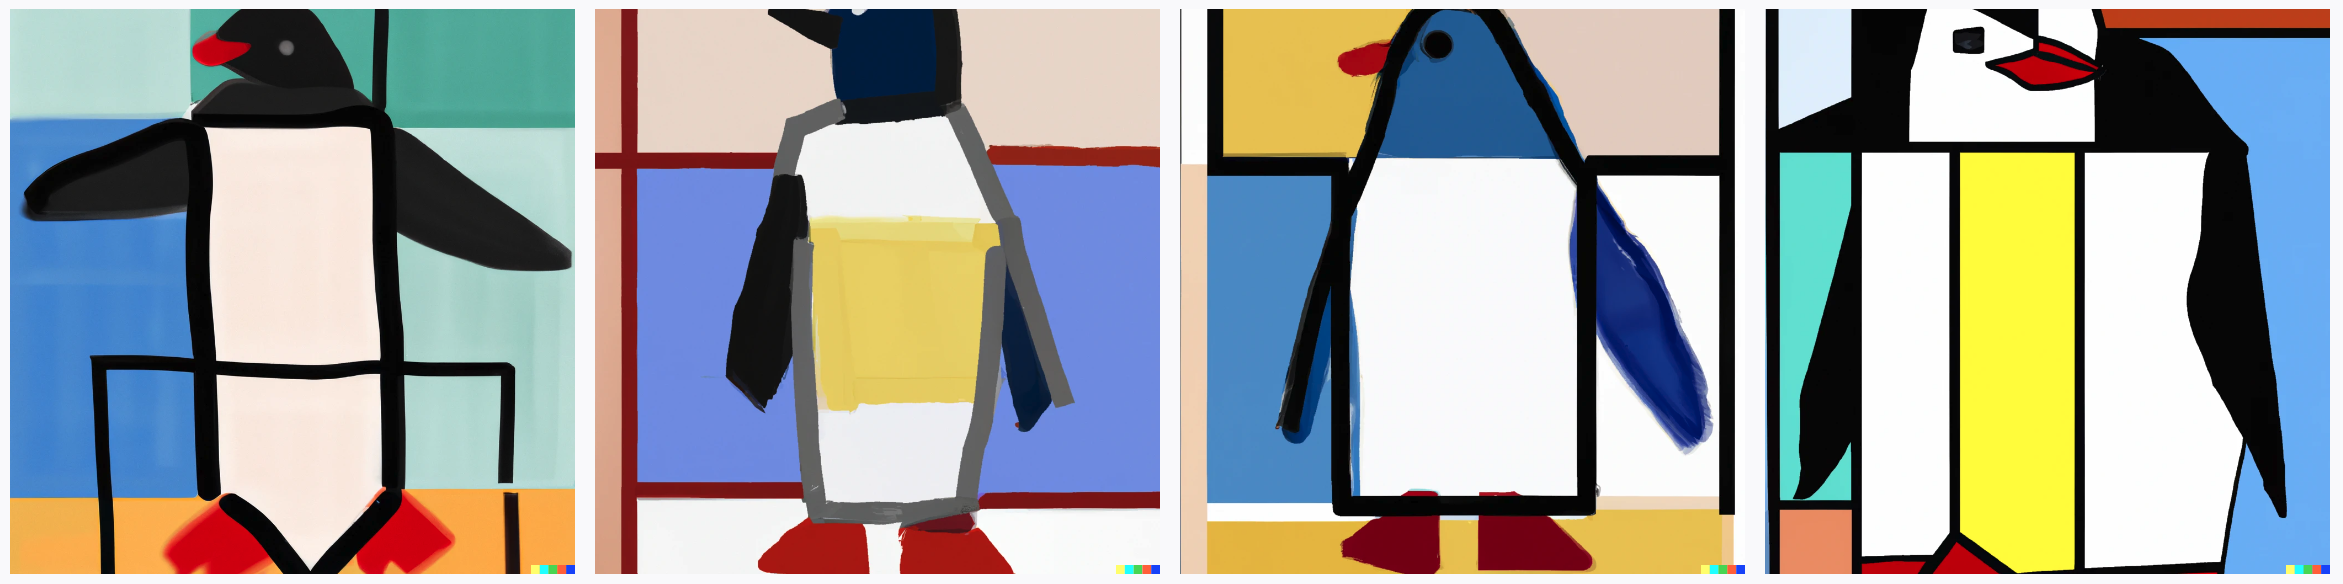
\includegraphics[width=\linewidth]{figures/text_to_image/DALLE2 Painting of a penguin in the style of Piet Mondrian.png}
	\caption{
		DALL-E 2 generations for the prompt \emph{Painting of a penguin in the style of Piet Mondrian}.
		\href{https://en.wikipedia.org/wiki/Piet_Mondrian}{Piet Mondrian} (1872-1944) was a Dutch artist pioneering abstract art, his later paintings were reduced to simple geometric objects.
	}
	\label{fig:DALLE2_penguin_piet_mondrian}
\end{figure}

\begin{figure}
	\centering
	
\includegraphics[width=\linewidth]{figures/text_to_image/DALLE2 A watercolour drawing of a torus surface in 3-dimensional space on a dark background.png}
	\caption{
		DALL-E 2 generations for the prompt \emph{A watercolour drawing of a torus surface in 3-dimensional space on a dark background}.
	}
	\label{fig:DALLE2_watercolour_torus_dark_background}
\end{figure}

\noindent \textbf{References:}
\begin{itemize}
	\item Joint text and image space:
	\cite{DBLP:journals/corr/abs-2111-07180}
	
	\item \href{https://openai.com/blog/clip/}{CLIP: Connecting Text and Images};
	\cite{radford2021learning};
	CLIP (Contrastive Language-Image Pre-training) is a multimodal machine learning model that learns a joint space for words and images by training on a large-scale dataset of image-text pairs.
	CLIP can perform zero-shot image classification by comparing natural language descriptions with image features.
	
	\item Text-to-image model DALL-E 2 \cite{Ramesh2022HierarchicalTI}
\end{itemize}

%~~~~~~~~~~~~~~~~~~~~~~~~~~~~~~~~~~~~~~~~~~%
\section{Structure in Word Embeddings}
%~~~~~~~~~~~~~~~~~~~~~~~~~~~~~~~~~~~~~~~~~~%

% % % % % % % % % % % % % % % % % % % % % % % %
\subsection{Sentiment specific word embeddings}

Sentiment analysis is a challenging task that aims to extract the subjective attitude or emotion of a text.
Word embeddings, which can capture the semantic and syntactic information of words in a low-dimensional vector space, are not inherently designed to encode sentiment information.
They may fail to distinguish between words with similar meanings but different polarities.
For example, the words \texttt{good} and \texttt{bad} may have similar embeddings because they are both adjectives that describe quality, but they have opposite sentiments \cite{yu-etal-2017-refining}.
Therefore, researchers have proposed various methods to refine word embeddings based on sentiment lexicon, sentiment concepts \cite{wang2021sentimentconcept}, or sentiment labels to improve their performance on sentiment analysis tasks.

\noindent \textbf{References:}
\begin{itemize}
	\item Using sentiment aware word embeddings for emotion classification \cite{sentiment-aware-word-embedding-emotion-2019}.
	\item TweetEval dataset, which includes emotion recognition and sentiment analysis tasks \cite{barbieri-etal-2020-tweeteval}, the authors released their \href{https://huggingface.co/cardiffnlp/twitter-roberta-base-sentiment}{pre-trained RoBERTa models}.
	\item German sentiment classification with fastText and BERT embeddings \cite{guhr-etal-2020-training}.
	\item EmoWOZ \cite{DBLP:journals/corr/abs-2109-04919} is a task-oriented dialogue dataset annotated with emotions.
\end{itemize}


% % % % % % % % % % % % % % % % % % % % % % % %
\subsection{Bias in Word Embeddings}

Machine learning models inherit and amplify biases present in data, such as stereotypes and prejudice.
For example, word embeddings may associate certain occupations or attributes with specific genders, \cite{DBLP:journals/corr/BolukbasiCZSK16a}, such as \texttt{man : computer programmer :: woman : homemaker}, or \texttt{he : brilliant :: she : lovely}.
In other cases, they might rank different ethnic groups differently according to some sentiment.

Such biases can have negative impacts on downstream applications that rely on word embeddings, such as machine translation, sentiment analysis, information retrieval, etc.
Therefore, it is important to identify and mitigate bias in word embeddings before using them for natural language processing tasks.
Several methods have been proposed to debias word embeddings at different levels: by modifying the data sources, by applying post-processing techniques, or by incorporating bias-aware objectives into the learning process.

In a first attempt, to investigate gender bias systematically, \cite{DBLP:journals/corr/BolukbasiCZSK16a} take the seed pair $(v_\textup{he}, v_\textup{she})$ and find other couples of word vectors which have a difference vector that is similar to the seed vector.
The authors also provide methods for debiasing the embedding, but they argue that bias ultimately appears to come from the training data.

\noindent \textbf{References:}
\begin{itemize}
	\item Iterative nullspace projection to debias word embeddings \cite{ravfogel-etal-2020-null}.
	\item Visualizations of bias mitigation techniques \cite{DBLP:journals/corr/abs-2104-02797},
	their \href{https://github.com/tdavislab/verb}{code} for creating interactive demos is available on GitHub.
	\item Gender bias in the contextualized embeddings from ElMo \cite{zhao-etal-2019-gender}.
	\item Bias in BERT embeddings \cite{kurita-etal-2019-measuring}.
	\item Debiasing contextualized embeddings \cite{kaneko-bollegala-2021-debiasing}.
\end{itemize}

%~~~~~~~~~~~~~~~~~~~~~~~~~~~~~~~~~~~~~~~~~~~~~~~~%
\section{Word Embeddings in Dialogue Systems}
%~~~~~~~~~~~~~~~~~~~~~~~~~~~~~~~~~~~~~~~~~~~~~~~~%


% % % % % % % % % % % % % % % % % % % % % % % % % % % % %
\subsection{Applications of Word Embeddings in Task-oriented Dialogue Systems}

A \emph{task-oriented dialogue system} is a computer system that can communicate with a human via natural language to help them complete a specific task, such as booking a ticket, ordering food or scheduling a call.
Task-oriented dialogue systems are different from chatbots that aim to have open-ended conversations with humans for entertainment or social purposes.
Task-oriented dialogue systems are more focused on achieving a clear goal and providing relevant information to the user.

A task-oriented dialogue system typically consists of four main components:

\begin{enumerate}
	\item \emph{Natural Language Understanding (NLU)}:
	This component is responsible for analyzing the user’s input and extracting relevant information, such as intents (what the user wants to do) and entities (what the user refers to).
	For example, if the user says ``I want to book a flight to Paris for next week'', the NLU component should identify the intent as booking a flight and the entities as ``Paris'' and ``next week''.
	Word embeddings improve the natural language understanding component by enabling it to handle synonyms, paraphrases, out-of-vocabulary words and cross-lingual inputs.
	\item \emph{Dialogue State Tracking (DST):}
	This component is responsible for keeping track of the current state of the dialogue, such as what information has been provided by the user and what information is still missing.
	For example, if the user has specified their destination but not their departure date, the DST component should store this information and update it accordingly.
	Word embeddings enhance the dialogue state tracking component by allowing it to compare user inputs and system outputs based on their semantic similarity.
	\item \emph{Policy:}
	This component is responsible for deciding what action to take next based on the current state of the dialogue.
	For example, if some information is missing from the user’s request, the policy component should decide to ask a clarifying question.
	If all the information is available, the policy component should decide to confirm or execute the request.
	Word embeddings facilitate the policy component by enabling it to learn from diverse data sources and generalize to unseen scenarios.
	\item \emph{Natural Language Generation (NLG):}
	This component is responsible for generating an appropriate response in natural language based on the action decided by the policy component.
	For example, if the policy component decides to ask for more information, then NLG should generate a question like “When do you want to depart?”.
	If the policy component decides to confirm or execute the request, then NLG should generate a response like “OK, I have booked your flight to Paris for next week.”.
	Word embeddings boost the natural language generation component by allowing it to produce fluent and diverse responses that match the user’s style and preferences.
\end{enumerate}

Nowadays, word embeddings are essential for building effective and robust task-oriented dialogue systems that can handle complex and dynamic user requests across different languages and domains.

Additionally, all of these components interface with an \emph{ontology}.
The ontology in a task-oriented dialogue system is a formal representation of the domain knowledge, concepts, and relations that are relevant for the task.
It defines the possible dialogue states, user intents, system actions, and slot values that can occur in the dialogue.
Ontologies can be either static or dynamic, depending on whether it is fixed or can change over time.

\begin{itemize}
	\item Domain: a general category of tasks or goals that the dialogue system can handle, such as restaurant booking, flight reservation, or weather information
	\item Slots: specific attribute or parameter that is relevant for the domain, such as cuisine type, departure date, or location
	\item Values: a possible filling for a slot, such as Italian, 15th of March, or London
\end{itemize}

For example, in the restaurant booking domain, the user may have the following dialogue with the system:

User: I want to book a table for two. System: What cuisine type do you prefer? User: Italian. System: When do you want to go? User: Tomorrow evening.

In this dialogue, the domain is restaurant booking, the slots are cuisine type and date, and the values are Italian and tomorrow evening.

\noindent \textbf{References:}
\begin{itemize}
	\item TripPy dialogue state tracker \cite{heck-etal-2020-trippy}
	\item \textcolor{magenta}{TODO} Add references
\end{itemize}

% % % % % % % % % % % % % % % % % % % % % % % % % % % % %
\subsection{Spoken Dialogue Systems and Automatic Speech Recognition}

Speech is a natural and efficient way for humans to communicate with each other and with machines.
However, speech alone is not enough to achieve effective communication; it also requires understanding of the meaning, context, and goals of the conversation.

Speech recognition and text-to-speech are essential components of a spoken dialogue system that enable the system to interact with the user using natural speech.
Speech recognition is the process of converting speech signals into text that can be processed by the system.
Speech recognition systems might use acoustic models, pronunciation dictionaries, and language models to decode speech inputs.

Text-to-speech is the process of converting text into speech signals that can be synthesized by the system.
Text-to-speech systems might use natural language generation, prosody modeling, and speech synthesis techniques to produce natural and expressive speech outputs.

These components need to be robust and adaptable to different domains, languages, accents, and environments.
They also need to handle out-of-vocabulary words, such as proper nouns and new words, that may not be recognized by the system ontology.

% % % %
\subsubsection{Whisper}

Whisper is a general-purpose speech recognition model developed by OpenAI \cite{radford2022robust}.
It is trained on a large dataset of diverse audio and is also a multitasking model that can perform multilingual speech recognition, speech translation, and language identification.

Whisper uses a Transformer sequence-to-sequence architecture that consists of an encoder and a decoder.
The encoder takes input audio that is split into 30-second chunks and converted into a log-Mel spectrogram.
The decoder predicts a sequence of tokens that represent various speech processing tasks, such as transcribing in the original language or translating to English.
These tasks are jointly represented by using special tokens that serve as task specifiers or classification targets.

\noindent \textbf{References:}
\begin{itemize}
	\item \href{https://openai.com/research/whisper}{OpenAI Whisper Blog post}
	\item OpenAI Whisper research paper \cite{radford2022robust}
\end{itemize}


% % % % % % % % % % % % % % % % % % % % % % % % % % % % %
\subsection{Aligning Language Models}

The \emph{GPT model family} is a family of language models that use deep learning techniques to generate natural language text.
They are built using several decoder blocks of the transformer architecture, which enables them to learn from large amounts of text data and produce coherent and diverse texts in an autoregressive manner.

\emph{Aligning language models} means training them to follow instructions given by humans, such as generating summaries, answering questions, or writing stories.
This can be done by using reinforcement learning from human feedback (RLHF), a method that rewards the model for producing outputs that match the user’s preferences
Alternatively, it can be done by self-instructing, a framework that generates instruction, input, and output samples from a language model itself and uses them to finetune the original model.

InstructGPT and ChatGPT are two examples of aligned language models that can follow instructions given by users. 
InstructGPT can generate texts for various tasks such as summarization, translation, or sentiment analysis.
ChatGPT can generate engaging and natural conversations for different domains such as gaming, sports, or movies.

\begin{itemize}
	\item \emph{Zero-shot learning} is a problem setup in machine learning where, at test time, a learner observes samples from classes which were not observed during training, and needs to predict the class that they belong to.
	For example, a zero-shot model can classify an image of a zebra without having seen any images of zebras during training.
	
	\item \emph{Few-shot learning} is a problem setup in machine learning where a learner needs to learn a new task from a very small number of labeled examples (typically less than 10 per class).
	For example, a few-shot learning model can recognize handwritten characters from different alphabets after seeing only one or few examples of each character.
\end{itemize}

\subsubsection{In-context learning (ICL)}

\emph{In-context learning (ICL)} is a problem setup in natural language understanding where a large pre-trained language model observes a test instance and a few training examples as its input, and directly decodes the output without any update to its parameters.
For example, an in-context learning model can perform sentiment analysis by conditioning on some input-output pairs that demonstrate the task.

\begin{lstlisting}
I love this movie. It's so funny and heartwarming. [positive]
This book is boring and poorly written. I don't recommend it. [negative]
The food was delicious and the service was excellent. [positive]
I don't like this song. It's too loud and annoying.
\end{lstlisting}


\textcolor{magenta}{TODO} Add references for in-context learning



\noindent \textbf{References:}
\begin{itemize}
	\item InstructGPT  \cite{ouyang2022training}
	\item Sparrow \cite{glaese2022improving}
	\item \href{https://openai.com/blog/chatgpt}{OpenAI ChatGPT blog post}
\end{itemize}

GPT-4 references:
\begin{itemize}
	\item GPT-4 technical report \cite{openai2023gpt4}
	\item The paper \cite{bubeck2023sparks} explores an early version of GPT-4, a large language model that can perform various tasks across domains without special prompting. The paper claims that GPT-4 exhibits more general intelligence than previous models and discusses its limitations and implications for artificial general intelligence.
\end{itemize}


%~~~~~~~~~~~~~~~~~~~~~~~~~~~~~~~~~~~~~~~~~~~~~~~~~~~~~~~~~~~~~~~~%
\section{Topological Data Analysis and Geometric Deep Learning}
%~~~~~~~~~~~~~~~~~~~~~~~~~~~~~~~~~~~~~~~~~~~~~~~~~~~~~~~~~~~~~~~~%

Geometric Deep Learning: Grids, Groups, Graphs, Geodesics, and Gauges is a book project \cite{bronstein2021geometric} that explores the geometric foundations of neural network architectures and their applications.
The book demonstrates how geometry can reveal the essential features and structure of the data and how it can inform the construction and improvement of neural architectures.
This perspective applies to various data domains such as images, sequences, graphs, and text, and various neural architectures such as CNNs, RNNs, GNNs, and Transformers.


% % % % % % % % % % % % % % % % % % % % % % % % % % % % %
\subsection{Geometry of the word embedding space}

\cite{mimno-thompson-2017-strange} find that in embeddings trained via skip-gram with negative sampling, the word vectors all point in roughly the same direction, i.e.\ they lie in a narrow cone.
This distribution is sometimes called \emph{anisotropy}.
The opposite of anisotropy is \emph{isotropy} where the vectors are directionally uniform.
The context vectors of the skip-gram model point in the other direction (which means that they have negative dot product with the mean of the word vectors).
In contrast to this, for GloVe the word and context vectors point in the same direction.

Method for finding words which are used differently in two text corpora:
train embedding on each corpus, find a mapping between the embedding spaces that produces an alignment (e.g.\ linearly via orthogonal Procrustes).
Then words which do not match well under this mapping appear to have different meanings.
Using historical texts, one can see how the meaning changes through time \cite{hamilton-etal-2016-diachronic}.

Different method for investigating alignment between different embedding spaces:
Train embeddings on two corpora separately, then for each word find the closest vectors in each embedding space.
If these differ a lot the embeddings are different \cite{gonen-etal-2020-simple}.

\noindent \textbf{References:}
\begin{itemize}
	\item Anisotropy can also be studied in contextualized word embeddings, see \cite{ethayarajh-2019-contextual}, where Ethayarajh defines measures of isotropy and compares those between the embedding models ELMo, BERT and GPT-2.
	\item \cite{cai2021isotropy} argue while contextual embeddings might appear anisotropic on first sight, they contain clusters and manifolds that reflect isotropy.
	\item \cite{rajaee-pilehvar-2021-cluster} present clustering based approaches for mitigating the anisotropy in contextual word embedding spaces.
	\item For isotropy in sentence embeeddings see \cite{li-etal-2020-sentence}.
	\item \cite{nakashole-flauger-2018-characterizing} observe that mappings between semantic spaces usually are only locally linear, and not globally linear.
\end{itemize}


% % % % % % % % % % % % % % % % % % % % % % % % % % % % %
\subsection{Embeddings in Curved Geometries}

Many real-world data sets have complex structures that cannot be adequately captured by Euclidean vector spaces.
For example, images of faces can be seen as points on a high-dimensional manifold that is curved and nonlinear.
To learn meaningful representations of such data, we need to take into account the \emph{intrinsic geometry} of the underlying \emph{manifold}.
\emph{Riemannian manifold learning (RML)} is a framework that aims to do this by using concepts and tools from Riemannian geometry.
RML assumes that the input high-dimensional data lie on an intrinsically low-dimensional Riemannian manifold, and seeks to construct coordinate charts that preserve the geodesic distances and local neighborhoods of the data points. 
By doing so, RML can reveal the latent structure of the data and enable various applications such as dimensionality reduction, clustering, classification, visualization and more.

Important keyword in this context include:
\begin{itemize}
	\item \emph{Manifolds}:
	A manifold is a topological space that is locally Euclidean, meaning that around every point, there is a neighborhood that looks like a flat space of some dimension.
	For example, a sphere is a two-dimensional manifold because any small patch on its surface can be flattened into a plane.
	Manifolds can be used to model complex data sets that have some underlying structure or smoothness. 
	\item \emph{Geodesics}:
	A geodesic is the shortest path between two points on a curved surface or manifold.
	For example, on a sphere, the geodesics are the great circles.
	Geodesics can be used to measure distances and angles on manifolds, and to define notions of curvature and parallel transport.
	\item \emph{Riemannian optimization}:
	Riemannian optimization is a branch of optimization that deals with finding optimal solutions on manifolds.
	It generalizes classical optimization methods such as gradient descent and Newton’s method by taking into account the geometry of the manifold.
	Riemannian optimization can be used to solve problems such as matrix factorization, low-rank approximation, principal component analysis and more on manifolds.
\end{itemize}

\textcolor{magenta}{TODO} Add references for Riemannian manifold learning

% % % % % %
\subsubsection{Positively Curved Spaces: Spherical Embeddings}

Euclidean embeddings might impose some limitations such as linearity and orthogonality.
Spherical Word Embeddings \cite{Meng2019SphericalTE} are an alternative approach that learns word vectors on a unit sphere, where the angle between two vectors reflects their similarity.
Spherical word embeddings can overcome some of the drawbacks of Euclidean word embeddings, such as being more flexible and expressive, being able to model antonyms and polysemous words better, and being more robust to noise and outliers.
Spherical word embeddings can also be extended to learn paragraph or document embeddings on a sphere, which can improve various downstream tasks such as document clustering and classification.

% % % % % %
\subsubsection{Negatively Curved Spaces: Hyperbolic Embeddings}

We can embed in so-called \emph{negatively curved spaces}, which are also known as \emph{hyperbolic embeddings}.
The geometry of these spaces allows a more efficient representation of tree-like structures and hierarchies, as was observed in \cite{DBLP:journals/corr/NickelK17}.
See also this \href{https://bjlkeng.github.io/posts/hyperbolic-geometry-and-poincare-embeddings/}{blog post} discussing the paper, and \href{https://rare-technologies.com/implementing-poincare-embeddings/}{this blog post} with implementation details.
In our case, where we associate words to points in a hyperbolic space, these are called \emph{hyperbolic word embeddings} (which can be constructed e.g.\ with Poincar{\'e} GloVe \cite{DBLP:journals/corr/abs-1810-06546}).
Further references include an earlier paper on hyperbolic text embeddings \cite{DBLP:journals/corr/abs-1806-04313},
these in turn were inspired by hyperbolic image embeddings \cite{DBLP:journals/corr/abs-1904-02239}.
There is also a proposed hyperbolic version of fastText \cite{zhu-etal-2020-hypertext}.
One can probe the contextualized embeddings of a BERT model by mapping into a hyperbolic space \cite{DBLP:journals/corr/abs-2104-03869}, and analyzing the structure of the projected data.

% % % % % % % % % % % % % % % % % % % % % % % % % % % % %
\subsection{Topological Data Analysis}

In \emph{Representation learning} we try to find a compact and dense representation of the data that captures its underlying structure, patterns, and relationships.
\emph{Point clouds} $X \subset \mathbb{R}^{N}$ are often the outcome of this process, as they allow for representing unordered collections of data units.

\emph{Topological Data Analysis (TDA)} \cite{carlsson2022topologicaldataanalysis} is a recently developed mathematical framework for understanding and simplifying complex data point clouds by capturing their essential \emph{shape}.
Some characteristic shapes of point clouds are illustrated in \Cref{fig:topological_data_analysis_collection}.
The \emph{shape of data} can mean the global structure or patterns of data that are invariant to transformations such as scaling, rotation, translation, or noise.
For example, a circle and an ellipse have the same shape because they can be transformed into each other by stretching or shrinking. 
Similarly, a spiral and a helix have the same shape because they can be transformed into each other by bending or twisting.

\emph{Topology} is a branch of mathematics that studies the properties of shapes that are preserved under continuous deformations.
TDA can provide insight into the shape of data by extracting features such as loops, holes, clusters, etc. that are robust to noise and occur in different dimensionality.

\textcolor{magenta}{TODO} Edit

\begin{itemize}
	\item Regression:
	Identify the relationship between a dependent variable and one or multiple independent variables.
	Applications include linear \emph{dimensionality reduction techniques} such as PCA.
	\item Clustering:
	Identify groups of similar data points.
	For instance, \emph{Single Linkage Clustering} groups data points based on the minimum distance between two points in a cluster.
	\item Periodic data:
	Cyclic patterns can appear in time series (daily patterns of human behavior, seasonal fluctuations in the stock market, annual changes in weather patterns, ...).
	Expressing the data in terms of a circular coordinate, it becomes easier to see patterns in the data that may not be immediately apparent otherwise.
	See \Cref{fig:coil_20,fig:coil_20_tsne}
\end{itemize}

\begin{figure}
	\centering
	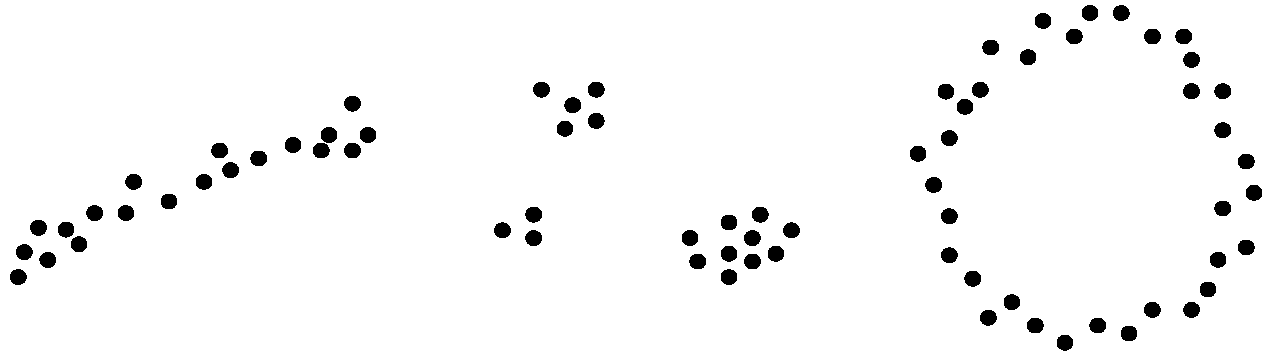
\includegraphics[width=0.8\linewidth]{figures/topological_data_analysis/topological_data_analysis_collection}
	\caption{
		Collection of various shapes of point clouds.
		\label{fig:topological_data_analysis_collection}
	}
\end{figure}

\begin{figure}[ht]
	\begin{minipage}[b]{0.55\linewidth}
		\centering
		% image from \cite{shi2014adaptive}
		% Jun Shi, Zhiguo Jiang, Hao Feng
		% Adaptive Graph Embedding Discriminant Projections
		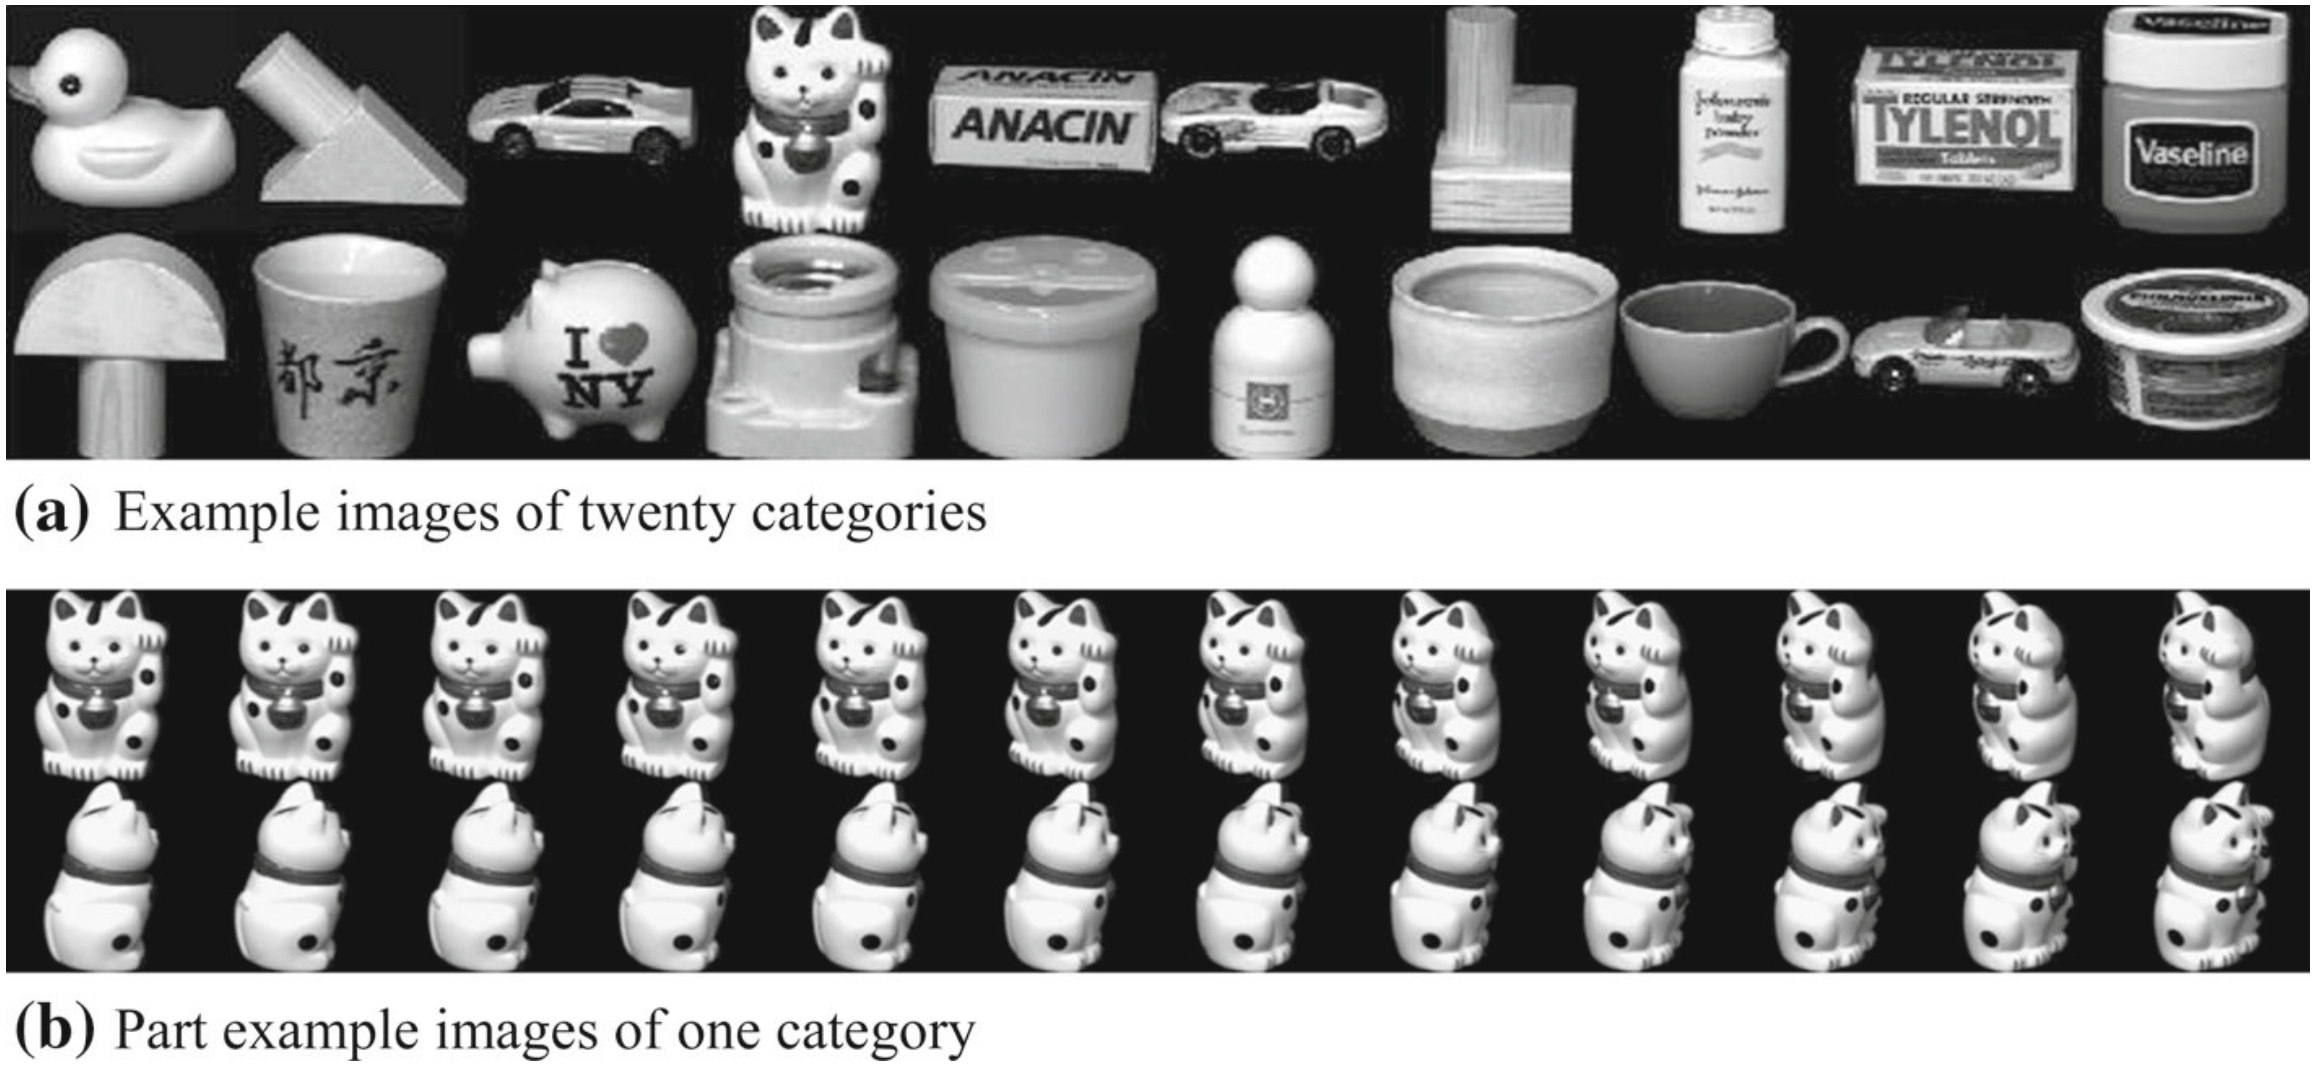
\includegraphics[width=1.0\linewidth]{figures/topological_data_analysis/coil_20_adaptive_graph_embedding_discriminant_projections}
		\caption{
			\href{https://www.cs.columbia.edu/CAVE/software/softlib/coil-20.php}{COIL-20 dataset}
			($128 \times 128$ grayscale images, twenty objects with 72 poses each)
		}
		\label{fig:coil_20}
	\end{minipage}
	\hfill
	\begin{minipage}[b]{0.4\linewidth}
		\centering
		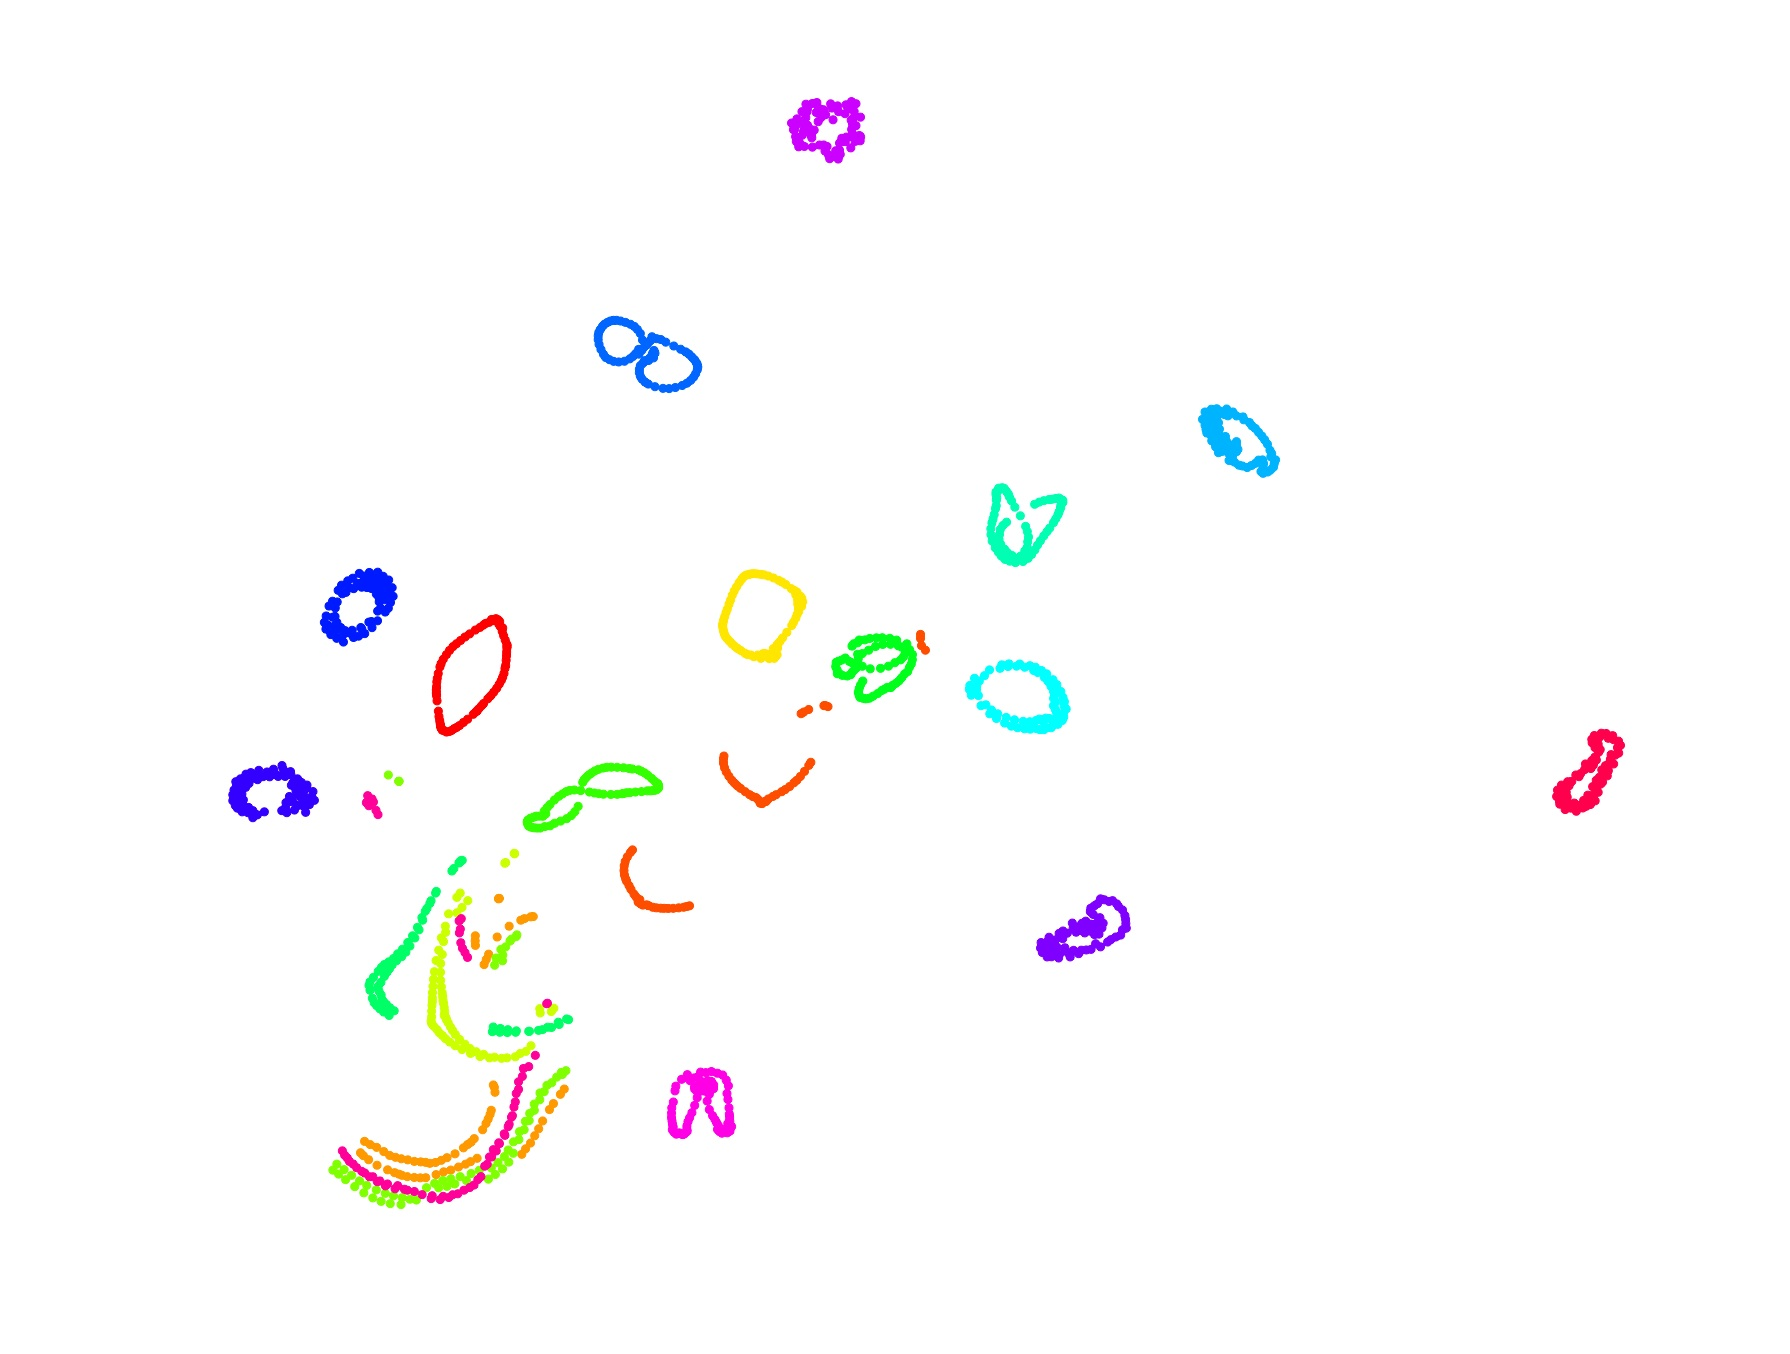
\includegraphics[width=1.0\linewidth]{figures/topological_data_analysis/coil_20_tsne_van_der_maaten}
		\caption{
			\href{https://lvdmaaten.github.io/tsne/}{2-dimensional $t$-SNE projection}
		}
		\label{fig:coil_20_tsne}
	\end{minipage}
\end{figure}

Topological Data Analysis is particularly useful in the analysis of high-dimensional data, where traditional regression methods may struggle because \emph{the best approximating shape might not be known a priory.}
For an illustration of the types of shapes underlying the data clouds in \Cref{fig:topological_data_analysis_collection}, have a look at \Cref{fig:topological_data_analysis_collection_with_shapes}.

\begin{figure}
	\centering
	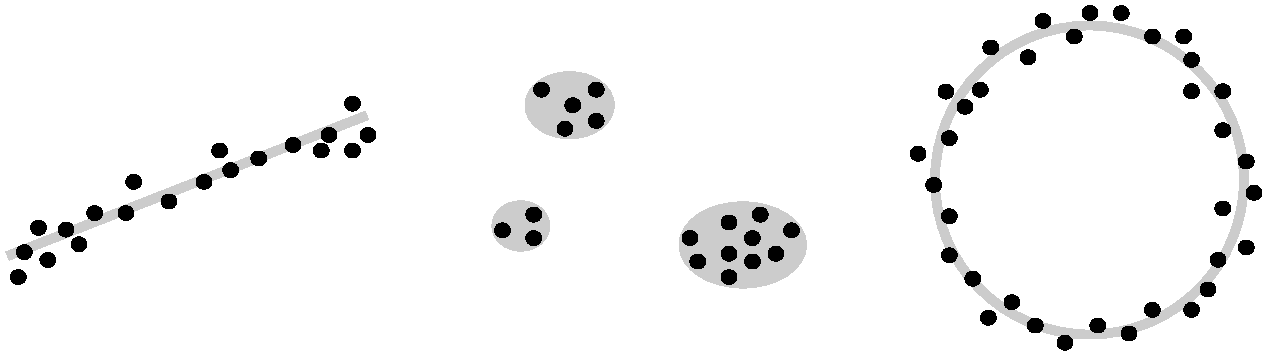
\includegraphics[width=0.95\linewidth]{figures/topological_data_analysis/topological_data_analysis_collection_with_shapes}
	\caption{
		Point clouds with approximating shapes.
		\label{fig:topological_data_analysis_collection_with_shapes}
	}
\end{figure}

% % % % % %
\subsubsection{Persistent Homology}

\emph{Vietoris-Rips complex:} \Cref{fig:vietoris_rips_complex}
Combinatorial description of the space via a \emph{simplicial complex}

\begin{center}
	\begin{figure}
		\centering
		\begin{tikzpicture}
			% \draw[step=1cm,color=gray] (0,0) grid (14,3.5); % Uncomment this to get some helpful grid lines
			\node[anchor=south west,inner sep=0] at (0,0){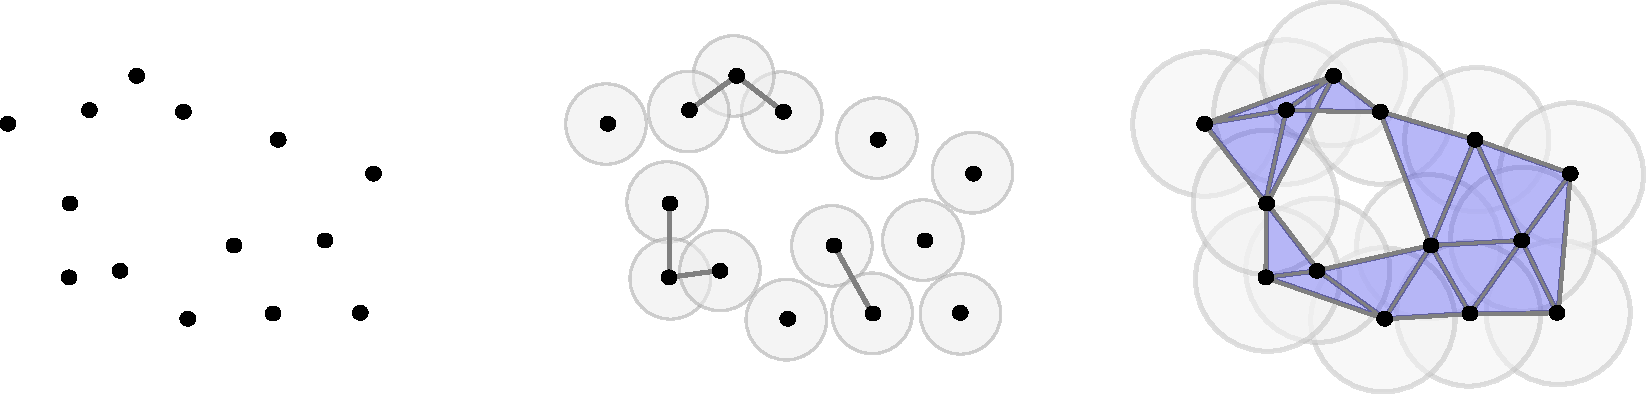
\includegraphics[width=0.95\linewidth]{figures/topological_data_analysis/vietoris_rips_complex.pdf}};
			\node at (3.0, 2.9) {\textcolor{black}{$\operatorname{VR}_{\varepsilon_{0}}(X)$}};
			\node at (8.0, 2.9) {\textcolor{black}{$\operatorname{VR}_{\varepsilon_{1}}(X)$}};
			\node at (13.0, 2.9) {\textcolor{black}{$\operatorname{VR}_{\varepsilon_{2}}(X)$}};
		\end{tikzpicture}
		\caption{
			Vietoris-Rips complex with various size scales
			\textcolor{magenta}{TODO} Fix labels
			\label{fig:vietoris_rips_complex}
		}
	\end{figure}
\end{center}

Idea of Persistent Homology:
Capture the evolution of topological features over \emph{different size scales} $\varepsilon_{i}$, to obtain insight into the intrinsic geometry of the data.

\begin{figure}
	\centering
	\begin{tikzpicture}
		% \draw[step=1cm,color=gray] (0,0) grid (10,6.5); % Uncomment this to get some helpful grid lines
		% Move the node slightly up in the y-direction to make room for the t_1 lable on the x-axis
		\node[anchor=south west,inner sep=0] at (0,0.6) {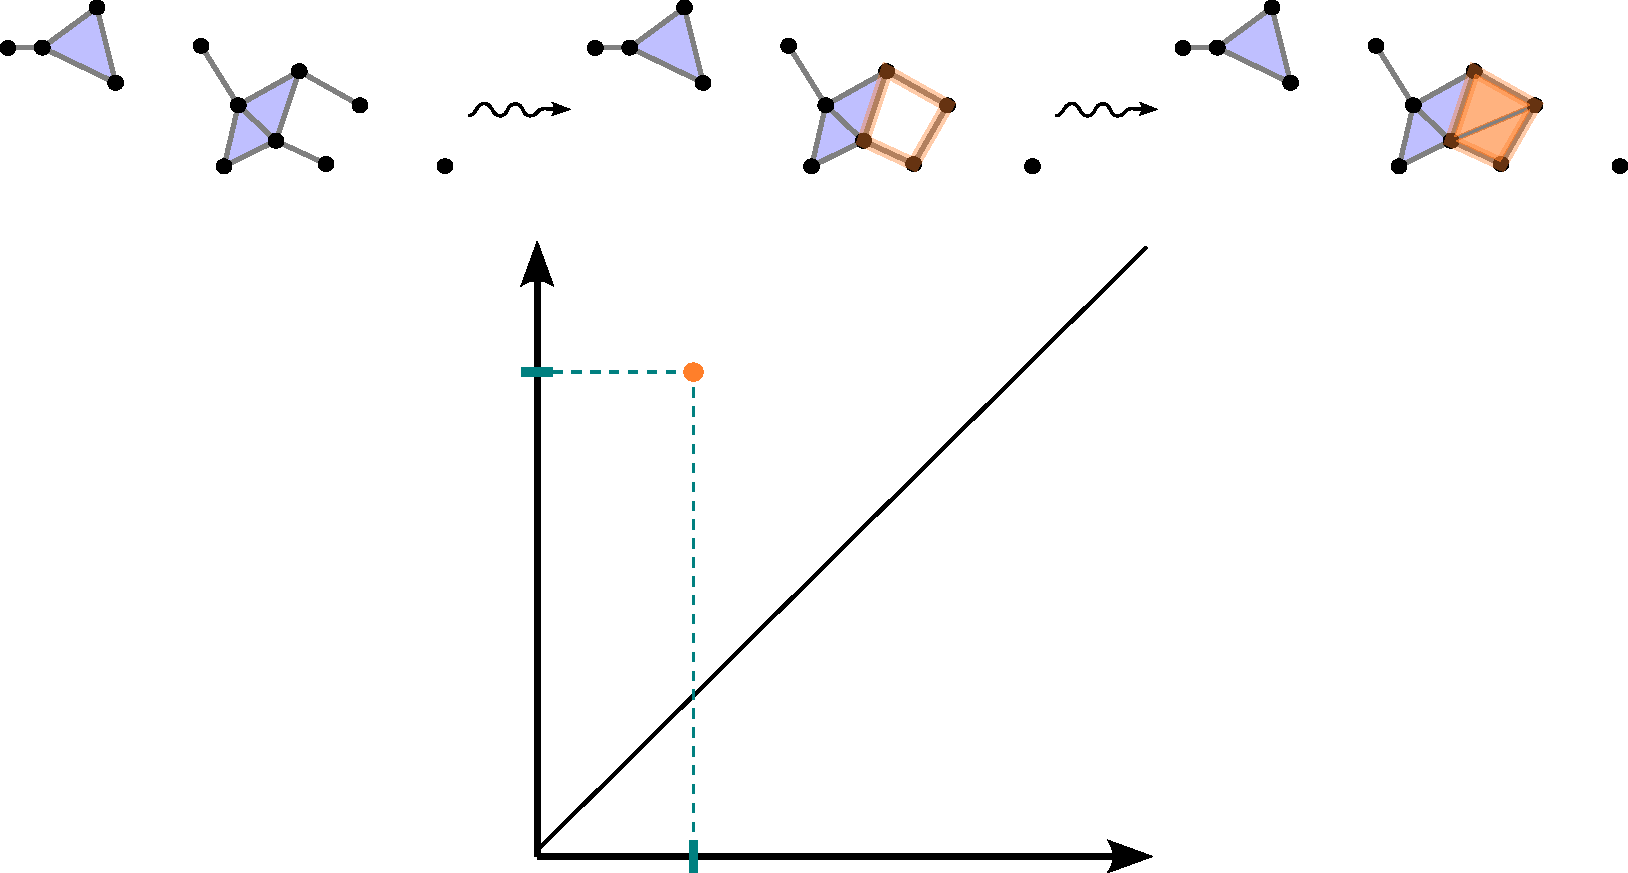
\includegraphics[width=0.55\linewidth]{figures/topological_data_analysis/persistence_diagram_with_filtered_complex.pdf}};
		% labels for the persistence diagram
		\node at (2.95, 3.65) {\textcolor{teal}{$t_{2}$}};
		\node at (4.25, 0.35) {\textcolor{teal}{$t_{1}$}};
		\node at (2.6, 4.3) {\textcolor{black}{death}};
		\node at (7.5, 0.7) {\textcolor{black}{birth}};
		% t_i above the simplicial complexes
		\node at (5.0, 6.1) {\textcolor{teal}{$t_{1}$}};
		\node at (8.5, 6.1) {\textcolor{teal}{$t_{2}$}};
	\end{tikzpicture}
	\caption{
		Filtered complex with persistence diagram.
		\textcolor{magenta}{TODO} Fix labels
		\label{fig:persistence_diagram}
	}
\end{figure}

Persistence diagrams: \Cref{fig:persistence_diagram}
Visual representations of the topological features and their \emph{lifespan} in a filtered simplicial complex.

Topological Deep Learning: \Cref{fig:topological_deep_learning}
Incorporate topological structures and insights into deep learning algorithms to improve their ability to capture and analyze complex relationships between data points.

\begin{itemize}
	\item Understanding of geometric and topological properties of data
	\item Insights into inner working of deep learning models
	\begin{itemize}
		\item The paper \cite{perez2022topological} presents a topological data analysis approach to text classification that uses BERT’s attention graphs as input, achieves comparable or better results than BERT on various tasks, and shows higher robustness and efficiency against adversarial attacks and attention head pruning.
		
	\end{itemize}
\end{itemize}

\begin{figure}
	\centering
	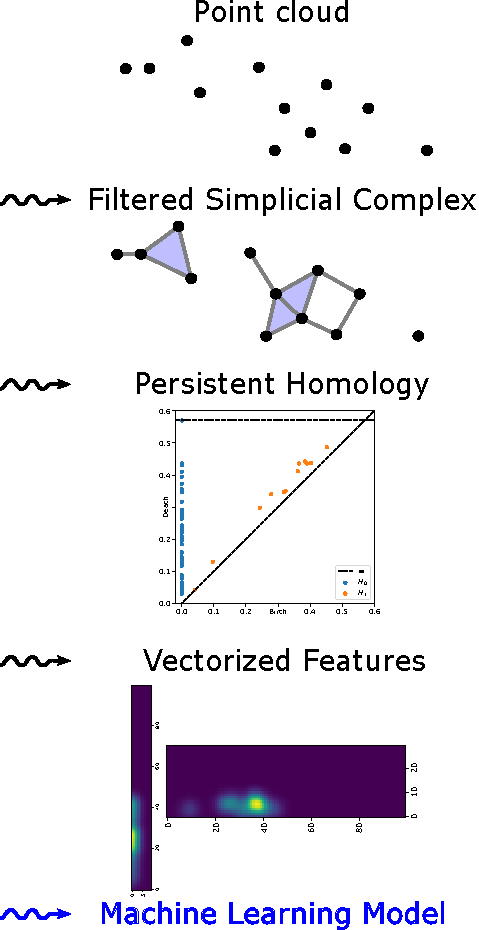
\includegraphics[width=0.2\linewidth]{figures/topological_data_analysis/topological_deep_learning}
	\caption{
		Topological Deep Learning Pipeline.
		\label{fig:topological_deep_learning}
	}
\end{figure}       


% % % % % %
\subsubsection{References for TDA}

There have been two main developments in Topological Data Analysis (TDA), which might lead to further interesting application of TDA to word embeddings in the future:
\begin{itemize}
	\item \emph{Persistent homology} is a description of the topological features of a space at various scales.
	Usually the data comes with a \emph{filtration}, and we compute the homology of the pieces which assemble into a \emph{persistence module}.
	These can be encoded into a \emph{bar-code}, which then is used in further machine learning pipelines.
	For example \cite{reinauer2021persformer} develop a Transformer model which takes persistence diagrams as input. 
	
	\item The MAPPER algorithm is a projection technique which also uses clustering to capture more of the global features of the dataset.
	An interesting projection choice is $t$-Stochastic Neighborhood Embedding ($t$-SNE, \cite{JMLR:v9:vandermaaten08a}).
\end{itemize}

Here are some general references for background reading on Topological Data Analysis:
\begin{itemize}
	\item \cite{murugan2019introduction}: Survey paper with an introduction to ``Topological Data Analysis for Physicists''.
	\item \cite{dey2021computational}: Book (draft) on Topological Data Analysis.
	\item Vidit Nanda's \href{http://people.maths.ox.ac.uk/nanda/cat/TDANotes.pdf}{Computational Algebraic Topology Notes}.
\end{itemize}


% % % % % % % % % % % % % % % % % % % % % % % % % % % % %
\subsection{Manifold Hypothesis and Singularities}

The \emph{Data Manifold Hypothesis} states that high-dimensional data lies on or near a low-dimensional structure called a manifold.\footnote{Manifold: Locally Euclidean topological space (plus some extra conditions)}
\Cref{fig:manifold_hypothesis}

\begin{itemize}
	\item \textbf{Consequence:} Most variation in the data can be captured by a small number of dimensions
	\item Important in dimensionality reduction techniques such as PCA, $t$-SNE, UMAP
	\newline
	$\leadsto$ Helps explain why these techniques often produce meaningful results
\end{itemize}

\begin{figure}
	\centering
	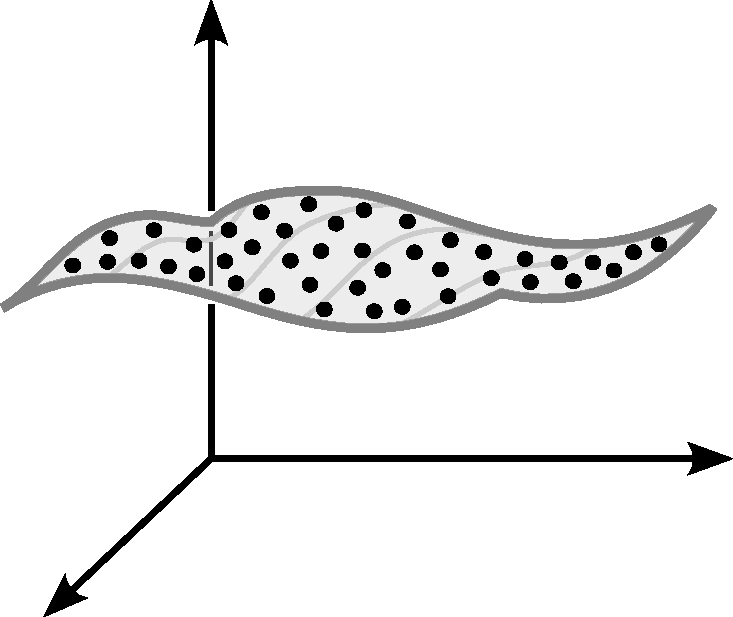
\includegraphics[width=0.4\linewidth]{figures/topological_data_analysis/manifold_hypothesis.pdf}
	\caption{
		Illustration of the Manifold Hypothesis.
		\label{fig:manifold_hypothesis}
	}
\end{figure}

Situations where the data \textbf{does not} have a low-dimensional structure and cannot be effectively mapped onto a lower-dimensional space:
\begin{itemize}
	\item Noise
	\item Few samples:
	it may not be possible to accurately estimate the underlying structure of the data due to the limited number of samples
	\item Multiple manifolds:
	If the data has multiple underlying structures, it may not lie on a single low-dimensional manifold, making it difficult to map onto a single reduced space.
	\item {\textbf{Singularities}}
\end{itemize}

\Cref{fig:manifold_hypothesis_problems}

\begin{figure}
	\centering
	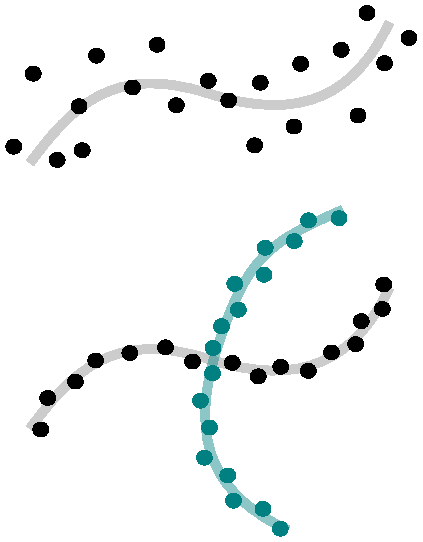
\includegraphics[width=0.35\linewidth]{figures/topological_data_analysis/manifold_hypothesis_problems.pdf}
	\caption{
		Potential problems with the manifold hypothesis.
		\label{fig:manifold_hypothesis_problems}
	}
\end{figure}

\textcolor{magenta}{TODO}

% % % % % %
\subsubsection{Topological Polysemy and singularities in word embeddings}

The paper \cite{jakubowski2020topology} studies singular points in a fixed word embedding trained via fastText, see \Cref{fig:TPS_paper_screenshot} for an illustration.
They find that the dimension of the zeroth local homology group of a punctured neighborhood of a word correlates with the number of different meanings of a polysemous word.

\textcolor{magenta}{TODO}

\begin{figure}
	\centering
	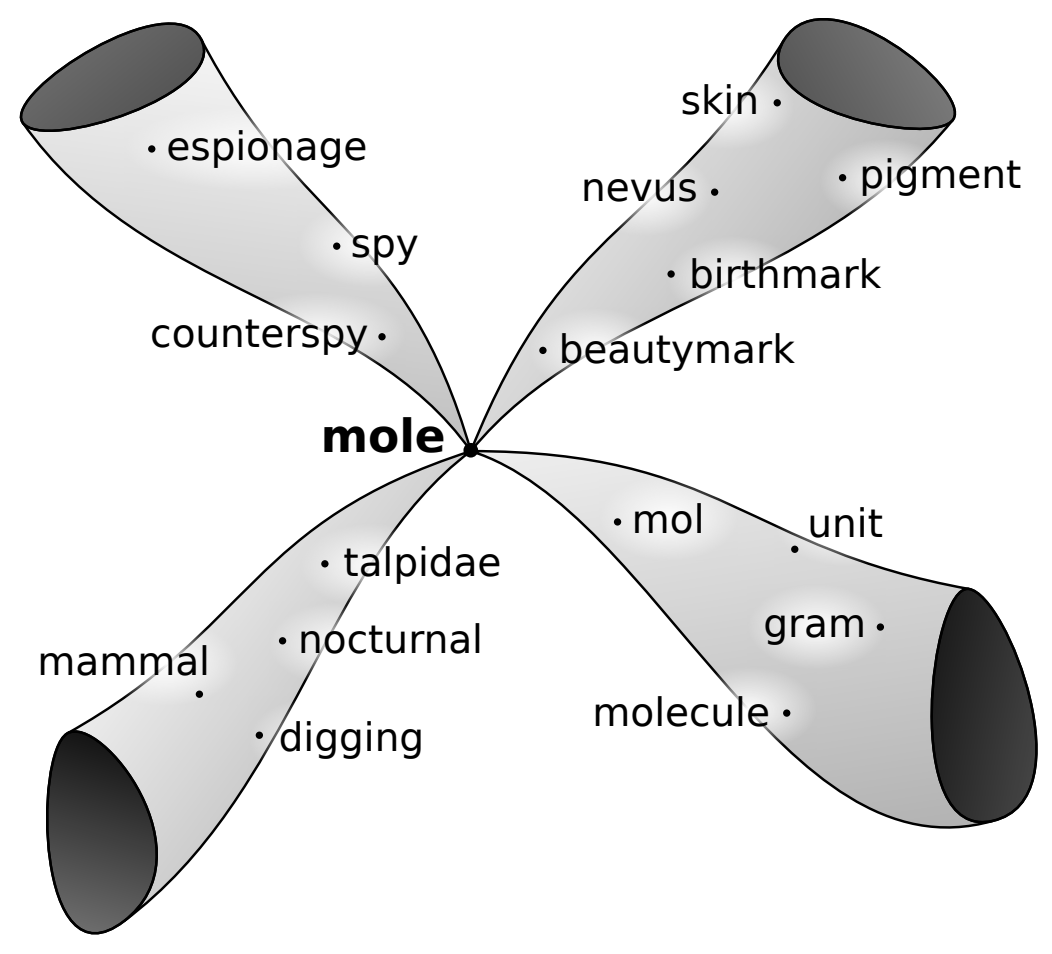
\includegraphics[width=0.35\linewidth]{figures/topological_data_analysis/TPS_paper_screenshot}
	\caption{
		Conceptual illustration of a singular point in a static word embedding in the neighborhood of the polysemous word `mole'.
		\label{fig:TPS_paper_screenshot}
	}
\end{figure}


\newpage
% % % % % % % % % %
% References
\printbibliography
% % % % % % % % % %


\newpage
% % % % % % % % % %
\appendix
% % % % % % % % % %


%~~~~~~~~~~~~~~~~~~~~~~~~~~~~~~~~~~~~~~~~~~~~~~~~%
\section{Prompts used in drafting the current notes}
\label{appendix:prompts}
%~~~~~~~~~~~~~~~~~~~~~~~~~~~~~~~~~~~~~~~~~~~~~~~~%

Some of the generative AI tools that were used to create these notes are ChatGPT and Bing Chat.
ChatGPT is a conversational model based on GPT-3.5 and GPT-4, which are large-scale language model that can generate coherent and diverse texts on various topics.
Bing Chat is a chat mode of Microsoft Bing search that can understand and communicate fluently in different languages, perform web searches, and generate creative content.

The \emph{prompts} are short sentences or questions that are typed into the chat box of these tools to elicit responses from them. 
Responses were then edited and integrated into the lecture notes as appropriate. 
The purpose of using these prompts is to enhance the quality and diversity of the lecture notes, as well as to demonstrate some of the capabilities and limitations of generative AI in natural language processing.
Prompts collected in this appendix are not meant to be comprehensive or exhaustive, but rather illustrative examples of how one can interact with these tools.

\Cref{table:examples_of_prompts} lists some of the prompts that were used, along with the corresponding tool name and response.
% The responses are marked with \generatedtext{code font} to indicate that they are generated by the tool and not by the authors of this document.

\begin{table}[h]
	\centering
	\begin{tabularx}{\textwidth}{ p{0.25\linewidth} p{1.5cm} X }
		\toprule
		Prompt & Tool & Example Response \\
		\midrule
		I am preparing lecture notes for a university class on word embedding spaces and representation learning in natural language processing with deep learning. Please write a short motivational paragraph in concise, scientific language, which explains the challenges behind capturing sentiment in word embeddings. 
		& Bing Chat (Mar 14 2023)
		& Here is a possible motivational paragraph for your lecture notes:
			Word embeddings are numerical representations of words that capture their semantic and syntactic information from contexts. They have been widely used for various natural language processing tasks, such as sentiment analysis. Sentiment analysis is the task of judging the tone or attitude of a document, such as a tweet, a song lyric, or a movie review. However, learning word embeddings that can capture sentiment information is challenging for several reasons [1][2][3][4]:
			Word embeddings are typically learned from large corpora of general texts, which may not reflect the specific domain or genre of the documents to be analyzed. For example, the word “sick” may have a negative connotation in a health-related corpus, but a positive one in a slang corpus.
			Word embeddings are usually context-independent, meaning that they assign the same vector to a word regardless of its surrounding words. However, the sentiment of a word may depend on its context. For example, the word “not” may reverse or modify the sentiment of the following word, such as “not bad” or “not good”.
			Word embeddings are often based on co-occurrence statistics, which may not capture subtle nuances or implicit meanings of words. For example, the word “fine” may have different sentiments depending on how it is used or pronounced, such as “I’m fine” or “Fine!”.
			Therefore, developing word embeddings that can effectively encode sentiment information is an important and active research area in natural language processing with deep learning. \\
		I am preparing lecture notes for a university class on word embedding spaces and representation learning in natural language processing with deep learning. Please write a short motivational paragraph in concise, scientific language, which explains the challenges behind capturing sentiment in word embeddings.
		& ChatGPT (Feb 13 2023)
		& Capturing sentiment in word embeddings is a complex task due to the inherent subjectivity and context-dependence of human emotions. The challenge lies in accurately capturing the nuances and variability of sentiment across different domains, languages, and cultural contexts, while avoiding bias and preserving semantic coherence. Additionally, the absence of explicit labeling of sentiment in training data and the trade-off between the dimensionality of the embedding space and its expressiveness further complicates the task. Despite these challenges, recent advances in representation learning with deep neural networks have shown promising results in capturing sentiment and related affective dimensions in word embeddings, enabling applications in sentiment analysis, emotion recognition, and natural language understanding.     \\ 
		G    & H      & I     \\ 
		\bottomrule
	\end{tabularx}
	\caption{Examples of prompts}
	\label{table:examples_of_prompts}
\end{table}



\end{document}
%%%%%%%%%%%%%%%%%%%%%%%%%%%%%%%%
%%%%%%%%%%%%%%%%%%%%%%%%%%%%%%%%